\chapter{Statistical mechanics}
\section{The Boltzmann distribution law}
\subsection{The canonical ensemble}
The canonical ensemble consists of cells of constant $V,T,N$, essentially a massive collection of bubbles sitting in a heat bath, and asks the question of how many of the bubbles will have the same energy. It is important to note that the particles within each cells are allowed to interact. In the derivation below note how we never assume the particles to be independent (interacting).
\subsubsection{Derivation}
Consider an isolated supersystem with a bath (surroundings) and a system we're interested in. We have
\begin{equation}
    E_{\text{tot}}=E_{\text{sys}}+E_{\text{bath}}.
\end{equation}
We now consider two states of the system, \textbf{A}, with $E_\text{bath,A}=E_{\text{tot}}$ and \textbf{B}, with the system in state $m$ with $E_m$. 
The number of microstates available to the supersystem $\Omega_{\text{tot}}$, is constant. We can write, from the postulate of equal probabilities, we can write
\begin{equation}
    P_m\propto\Omega_{\text{bath}}(E_{\text{tot}}-E_m)
\end{equation}
This can look superficially simple but let's think what it actually means: the postulate of equal probabilities only applies to the \emph{supersystem}, which is isolated. So we can only say that the probability of observing the \emph{system} with energy $E_m$ is proportional to the number of microstates that has the bath with that energy. The choice to use the perspective of the bath but not the system is arbitrary now, however a subsequent approximation makes it necessary. \par
To find the exact functional form of $\Omega_{\text{bath}}(E_{\text{bath}})$, we invoke the definition
\begin{equation}
    \diffp SU[V]=\frac{1}{T}
\end{equation}
Considering just the bath, we have
\begin{equation}
    \diff{\ln{\Omega}_{\text{bath}}(E_{\text{bath}})}{E_{\text{bath}}}=\frac{1}{kT}.
\end{equation}
Now we make the important approximation that, in the limit of $E_{\text{tot}}\gg E_m$, we can approximate the derivative with a simple geometric gradient
\begin{equation}
    \frac{\ln \Omega_{\text{bath}}(E_{\text{bath,B}})-\ln\Omega_{\text{bath}}(E_{\text{bath,B}})}{E_{\text{text,B}}-E_{\text{bath,A}}}=\frac{1}{kT}
\end{equation}
and this readily gives 
\begin{equation}
  \Omega_{\text{bath}}(E_{\text{tot}}-E_m)=\Omega_{\text{bath}}(E_{\text{tot}})\exp\lf(\frac{-E_m}{kT} \rt)
\end{equation}
and as $E_{\text{tot}}$ is fixed, we have
\begin{equation}
  P_m=B\exp\lf(\frac{-E_m}{kT} \rt)
\end{equation}
where $B$ is $1/q$, via the same normalisation argument.

\subsection{Derivation of Boltzmann distribution}
\subsubsection{Via a Lagrange multiplier}
We now derive the Boltzmann distribution law again, this time minimising a free energy. 
The problem we solve is essentially the same as the one in \Cref{chapter1}: 
we are given energy states $E_j$ from the physics of the problem, 
and we aim to compute the probabilities $p_j$ that the system is in $j$. \\
We now suppose that $(T,V,N)$ are held constant, with only one species of particles. 
The condition for \eqm is then 
\begin{equation}
\dif A=\dif U-T\dif S=0.
\end{equation}
This looks arbitrary but we can use any free energies as we have demonstrated in 
\Cref{free_energy}, minimising any of them under appropriate conditions 
is equivalent to maximising entropy. \\
Evidently now we need expressions for $\dif S$ and $\dif U$. 
We have the expression for entropy:
\begin{equation}
S(\bvec{p})=-k\sum^{t}_{j=1}p_j\ln p_j, 
\end{equation}
which readily gives
\begin{equation}
\dif S=\sum\diffp{S(\bvec{p})}{p_j}[p_{i\neq j}]=-k\sum^t_{j=1}(1+\ln p_j)\dif p_j.
\end{equation}
\begin{post}[Internal energy]
The internal energy is given as the average over all microscopic states:
\begin{equation}
U=\lgl E\rgl=\sum^{t}_{j=1}p_jE_j.
\end{equation}
\end{post}
We then have
\begin{equation}
\label{du_boltz}
\dif U=\dif \lgl E\rgl=\sum^{t}_{j=1} (E_j\dif p_j+p_j\dif E_j).
\end{equation}
\begin{post}[Energy levels]
Energy levels $E_j$ only depends on volume and number of particles, and unlike $U$ do not depend on $S$ and $T$:
\begin{equation}
E_j=E_j(V,N).
\end{equation}
\end{post}
This means 
\begin{equation}
\dif E_j=\diffp{E_j}{V}\dif V+\diffp{E_j}{N}\dif N=0.
\end{equation}
As both $V$ and $N$ are held constant, 
\begin{equation}
\dif E_j=0, 
\end{equation}
and \Cref{du_boltz} becomes
\begin{equation}
\dif U=\dif \lgl E\rgl=\sum^{t}_{j=1} E_j\dif p_j.
\end{equation}
Now we have our \textbf{objective function}:
\begin{equation}
\dif A=\dif \lgl E\rgl-T\dif S=0,
\end{equation}
and the \textbf{constraint function} is then the usual
\begin{equation}
\begin{aligned}
\sum^{t}_{j=1} p_j&=1\\
\sum^{t}_{j=1} \dif p_j&=0.
\end{aligned}
\end{equation}
We can then write our Lagrange multiplier as
\begin{equation}
\dif A=\sum^{t}_{j=1} \lf[E_j+kT(1+\ln p_j^*)+\lambda \rt]\dif p_j^*=0.
\end{equation}
Thie requires that
\begin{subequations}
\begin{align}
\ln p_j^*&=-\frac{E_j}{kT}-\frac{\lambda}{kT}-1\\
p_j^*&=e^{-E_j/kT}e^{-(\lambda/kT)-1}. \label{pstarred}
\end{align}
\end{subequations}
As $p_j$'s sum to $1$,
\begin{equation}
\label{probsum}
\sum^{t}_{j=1} e^{-E_j/kT}e^{-(\lambda/kT)-1}=1,
\end{equation}
we can divide \Cref{probsum} through \Cref{pstarred} to eliminate $\lambda$, 
and yield the
\begin{thrm}[Boltzmann distribution law]
The law states that
\begin{equation}
\label{bdl}
p_j^*=\frac{\exp(-E_j/kT)}{\sum^t_{j=1}\exp(-E_j/kT)}\equiv\frac{1}{q}\exp(-E_j/kT).
\end{equation}
where $q$ is the partition function and $E_j$ is the energy of \emph{state} $j$. When multiple states have the same energy \ie degenerate, it is convenient to merge them into \emph{levels} of degeneracy $g_i$:
\begin{equation}
  p_i=\frac{g_i}{q}\exp \lf(\frac{-E_i}{kT} \rt)
\end{equation}
\end{thrm}
The Boltzmann distribution law is just a consequence of maximising entropy: given 
total energy, more molecules would have lower energy 
rather than a few having high energies and the rest having zero, 
to maximise total multiplicity.
\subsubsection{From the canonical distribution}
The Boltzmann distribution essentially arise from the canonical distribution when the particles are non-interacting, basically, we now can say that $Q_N=q^N/N!$ for indistinguishable particles, which is what we assume all along anyway. An outline of the proof is given below:\par
If we assume the particles are independent and non-interacting, we can write
\begin{equation}
  Q_N=\frac{q^N}{N!}
\end{equation}
and with 
\begin{equation}
  U=kT^2\diffp {\ln Q_N}{T}
\end{equation}
we can write
\begin{equation}
  U=NkT^2\frac{1}{q}\diffp qT[V]
\end{equation}
where 
\begin{equation}
  q=\sum_i\exp \lf(\frac{-\ep_i}{kT} \rt)
\end{equation}
So 
\begin{equation}
  \diffp qT[V]=\frac{1}{kT^2}\sum_i\ep_i\exp \lf(\frac{-\ep_i}{kT} \rt)
\end{equation}
Substituting this back into the expression for internal energy, we have
\begin{equation}
  U=\frac{N}{q}\sum_i\exp\ep_i\exp \lf(\frac{-\ep_i}{kT} \rt)
\end{equation}
But internal energy is also just the expectation value:
\begin{equation}
  U=\sum_i n_i\ep_i
\end{equation}
So clearly we can identify
\begin{equation}
\begin{aligned}
  n_i&=\frac{N}{q}\exp \lf(\frac{-\ep_i}{kT} \rt)\\
  p_i&=\frac{1}{q}\exp \lf(\frac{-\ep_i}{kT} \rt)
\end{aligned}
\end{equation}
\subsection{Interpretation of partition function}
\subsubsection{Physical meaning of the partition function}
We introduced the partition function, but have not discussed why it's called `partition function'. 
The partition function is 
\begin{equation}
Q\equiv \sum^{t}_{j=1} e^{-E_j/kT}.
\end{equation}
However, it's more commonly expressed in terms of energy differences as experiments often yield those. 
It is then convenient to define the ground-state as zero, $E_1=0$, and write
\begin{equation}
Q=1+e^{-(E_2-E_1)/kT}+e^{-(E_3-E_1)/kT}+\cdots++e^{-(E_t-E_1)/kT}.
\end{equation}
The two forms are equivalent. \\
Now, when the energies for all energy levels are small, \textit{or} the temperature is high, all the states are equally populated and we have that 
\begin{equation}
\frac{E_j}{kT}\rightarrow0\ \imp\ Q\rightarrow t\ \imp\ p_j^*\rightarrow\frac{1}{t}.
\end{equation}
If all the \textit{non-ground state} energies approach infinity, or the temperature approaches zero, the particles can only occupy the ground state:
\begin{equation}
\frac{E_{j\neq1}}{kT}\rightarrow \inf\ \imp\ Q\rightarrow1\ \imp\ p_1^*\rightarrow1.
\end{equation}
In this casem only the ground state becomes \textit{effectively accessible}. \\
So we can see that the partition function gives the number of states that are \emph{effectively} accessible to the system, 
and the magnitude of $E_j/kT$ determines whether or not the state $j$ is \textit{effectively} accessible. 
But beware that the number of accessible states is always the same $t$ and is independent of system varibles as it is fixed by the physics of the situation. 
In contrast, $Q$ is a function of system variables such as $T$. 

\subsubsection{Distinguishability}
\begin{defi}[Distinguishability]
The distinction between distinguishable and indistinguishable particles lies in 
the de Broglie wavelength in comparison of typical particle separation of the 
type of particle in question, and \textit{not in whether the particles are identical or not}. \\
For example, two tennis balls can be identical but occupy distinct locations and can thus be distinguished. 
The same is true for particles fixed in a lattice, which occupy a relatively fixed position. \\
However, two electrons in the He atom have de Broglie wavelengths about the same or larger than the interelectronic separation, hence cannot be distinguished. 
The same goes for particles in a gas, for example. 
\end{defi}
Now we consider systems made of two independent, distinguishable particles $A$ and $B$. 
The energy levels are $E_j$ and is given as a sum of individual energy levels:
\begin{equation}
E_j=\epsilon_i^A+\epsilon_m^B.
\end{equation}
As the two particles are independent, they have independent partition functions,
\begin{equation}
q_A=\sum^{a}_{i=1} e^{-\epsilon_i^A/kT},
\end{equation}
and likewise for $B$. \\
The partition function for the system is the sum of Boltzmann factors $e^{-E_j/kT}$ over all $j=ab$ energy levels:
\begin{equation}
Q=\sum^{t}_{j=1} e^{-E_j/kT}=\sum^{a}_{i=1} \sum^{b}_{m=1} e^{-(\epsilon_i^A+\epsilon_m^B)/kT}=\sum^{a}_{i=1} \sum^{b}_{m=1} e^{-\epsilon_i^A/kT}e^{-\epsilon_m^B/kT}.
\end{equation}
Because the two paricles are distinguishable, all $j=ab$ energy levels are distinct and independent, for example, $A$ in level 26 and $B$ in level 53 is different from $B$ in 26 and $A$ in 53, hence we can write that
\begin{equation}
Q=\sum^{a}_{i=1} e^{-\epsilon_i^A/kT}\sum^{b}_{m=1} e^{-\epsilon_m^B/kT}=q_Aq_B, 
\end{equation}
and in general, for a system with $N$ distinguishable particles, 
\begin{equation}
Q=q^N.
\end{equation}
However, for indistinguishable particles, having $A$ in level 23 and $B$ in level 54 is exactly the same as the other way around, and the better way to specify this 
is to say that `one particle is in level 23 and another in level 54.' 
Therefore, if we were to count distinct energy levels, which is what the partition function is about, 
we should divide the count by $N!$
\footnote{This is an approximation as if the particles coincide on the same energy level, there will not be overcounting, but this is in reality often negligible as the number of accssible levels are usually much larger than number of particles.}:
\begin{equation}
Q=\frac{q^N}{N!}.
\end{equation}


\subsubsection{Gibb's paradox}
Another, and in my opinion, much better justification for dividing by $N!$ comes from \cite{vnd} 
which shows that the division is merely a redefinition and has no 
fundamental justification, it is there to reconcile the statistical mechanical 
and thermodynamical definitions of entropy, the differences of which was revealed 
by the Gibb's paradox, which provides for two isolated box 
with $N$ identical particles and $X$ accessible energy states, separated by an infinitely 
thin and isolating division. Let's call the system before and after removing the division $A$ and $B$, and 
the multiplicities are given as
\begin{subequations}
\begin{align}
S_A&=X^{2N}\\
S_B&=(2X)^{2N}.
\end{align}
\end{subequations}
The change in entropy is 
\begin{equation}
S_B-S_A=2kN\ln 2,
\end{equation}
but the change must be
\begin{equation}
S_B-S_A=\int^B_A \frac{\indiff Q}{T},
\end{equation}
as the gases remain in equilibrium the removal of division is a quasistatic process so the change \textit{must} be zero. 
This is the Gibb's paradox. To resolve it, we must realise that the definition of
\begin{equation}
S=k\ln W
\end{equation}
is for statistical mechanics and not for thermodynamics, and that, indeed the number
of accessible energy levels has increased but this does not correspond well with the usual notion of entropy, hence we need to redefine entropy as
\begin{equation}
S=k\ln\frac{W}{N!}.
\end{equation}
Now, the `new' multiplicities are 
\begin{subequations}
\begin{align}
W_A&=\frac{X^{2N}}{(N!)^2}\\
W_B&=\frac{(2X)^{2N}}{(2N)!}.
\end{align}
\end{subequations}
We apply Stiring's approximation under the assumption of the \textit{thermodynamic limit} of $N\rightarrow\inf$: 
\begin{equation}
\ln n!\approx n\ln n-n
\end{equation}
to show that
\begin{subequations}
\begin{align}
\ln W_A&=2N\ln X-2\ln N!\approx 2N\ln X-2N\ln N+2N \\
\ln W_B&=2N\ln 2X-2\ln (2N)!\approx 2N\ln 2X-2N\ln 2N+2N.
\end{align}
\end{subequations}
The two expressions are equal, and we have resolved the Gibb's paradox. 
This also provides another justification for dividing the partition function by $N!$. 

\subsection{Applications of the Boltzmann distribution}
\subsubsection{Population of states}
We go through partition functions in great detail in \Cref{nststatmech}, and we use the results from there:
\paragraph{Populations of vibrational energy levels}
For a simple harmonic oscillator, the energy levels, with the lowest level set to 0, are
\begin{equation}
  \ep_{\nu}=\nu h\nu_0
\end{equation}
and 
\begin{equation}
  q'_{\text{vib}}=\frac{1}{1-\exp(-h\nu_0/kT)}
\end{equation}
so we have
\begin{equation}
  p_{\nu}=\lf[1-\exp\lf(\frac{-\theta_{\text{vib}}}{T}\rt) \rt]\exp \lf(\frac{-\nu\theta_{\text{vib}}}{T} \rt)
\end{equation}
\paragraph{Populations of rotational energy levels}
For a rigid rotor, the levels are
\begin{equation}
  \ep_J=BJ(J+1)
\end{equation}
and the levels have degeneracies of $(2J+1)$, so
\begin{equation}
  p_J=\frac{2J+1}{q_{\text{rot}}}\exp \lf(\frac{-BJ(J+1)}{kT} \rt)
\end{equation}
In the high temperature limit (reached at very low actual temperatures, so almost always valid), 
\begin{equation}
  q_{\text{rot}}=\frac{T}{\sigma\theta_{\text{rot}}}
\end{equation}
where $\theta_{\text{rot}}=B/k$, we have
\begin{equation}
  p_J=\frac{\sigma\theta_{\text{rot}}}{T}(2J+1)\exp \lf(\frac{-\theta_{\text{rot}}J(J+1)}{T} \rt)
\end{equation}
The degeneracy term wins out the exponential form at small $J$ and so intensity increases at first, but eventually tails out. The maximum can be found by setting $\diff{p_J}/{J}=0$, which gives
\begin{equation}
  J_{\text{max}}=\sqrt\frac{T}{2\theta_{\text{rot}}}-\frac{1}{2} 
\end{equation}
\subsubsection{Density of states}
The density of states $D(\ep)$ is the number of states per energy, or $D(\ep)\dif\ep$ is the number of states between $\ep$ to $\ep+\dif\ep$. It is formally the derivative of number of states, $W(\ep)$, which gives the number of states up to $\ep$:
\begin{equation}
  D(\ep)=\diff{W(\ep)}{\ep}
\end{equation}
We consider the very densely packed case of translational energy states: in a cubical box of side $a$, the energy levels are
\begin{equation}
  E_{n_x,n_y,n_z}=(n_x^2+n_y^2+n_z^2)\frac{h^2}{8ma^2}
\end{equation}
This is reminiscent of the Cartesian expression for a sphere, with $n_x^2+n_y^2+n_z^2$ the squared radius, so the `radius' is given as 
\begin{equation}
  n_{\text{max}}=\lf(\frac{8ma^2\ep}{h^2} \rt)^{1/2}
\end{equation}
However, only the octant corresponding to positive $(x,y,z)$ can be taken as $n_i$'s are nonzero, so the number of states are
\begin{equation}
  W(\ep)=\frac{1}{8}\times\frac{4}{3}\pi n_{\text{max}}^3=\frac{\pi}{6}\lf(\frac{8m\ep}{h^2} \rt)^{3/2}V
\end{equation}
where we wrote $a^3$ as $V$. $D(\ep)$ soon follows:

\begin{thrm}[Density of translational states in a box]
For a cubical box with volume $V$, $D(\ep)$ is given as 
\begin{equation}
  D(\ep)=\diff{D(\ep)}{\ep}=\frac{\pi}{4}\lf(\frac{8m}{h^2} \rt)^{3/2}\ep^{1/2}V
\end{equation}
\end{thrm}
This is a result that will come in handy when we constider the free electron gas model of metal bonding.
\subsubsection{Non-equilibrium states}
The population ratio between states is given as 
\begin{equation}
  \frac{n_1}{n_0}=\exp \lf(\frac{-\Delta\ep}{kT} \rt)
\end{equation}
It is possible to excite population from the lower energy level selectively by methods such as intense radiation, such that $n_1>n_0$ and the temperature is temporarily negative. This is called a \emph{population inversion}, which is important in the working of lasers.
\subsubsection{Maxwell-Boltzmann distribution of velocities}
We adopt the assumptions of the kinetic theory that gas particles can be 
treated as perfect Newtonian particles. The kinetic energy, which is the total energy is given by 
\begin{equation}
\epsilon(v)=\frac{1}{2}mv^2.
\end{equation}
According to the Boltzmann law, the probability $p(v_x)$ that a particle in a container at constant volume and temperature will have volcity $v_x$ in the $x$ direction is 
\begin{equation}
p(v_x)=\frac{e^{-\epsilon/kT}}{\intinf e^{-\epsilon/kT}\dif v_x}, 
\end{equation}
where $\dif v_x$ serves the same role as the rolling index $j$ in \Cref{bdl}. 
We write further that
\begin{subequations}
\begin{align}
p_(v_x)&=\frac{e^{-mv_x^2/2kT}}{\intinf e^{-mv_x^2/2kT}\dif v_x}\\
&=\lf(\frac{m}{2\pi kT} \rt)^{1/2}e^{-mv_x^2/2kT}
\end{align}
\end{subequations}
The \textit{mean-square} velocity is
\begin{subequations}
\begin{align}
\lgl v_x^2\rgl&=\intinf v_x^2p(v_x)\dif v_x\\
&=\lf(\frac{m}{2\pi kT} \rt)^{1/2}\intinf v_x^2e^{-mv_x^2/2kT}\dif v_x\\
&=\lf(\frac{m}{2\pi kT} \rt)^{1/2}\lf(\frac{kT}{m} \rt)\lf(\frac{2\pi kT}{m} \rt)^{1/2} \\
&=\frac{kT}{m}.
\end{align}
\end{subequations}
This means that the average kinetic energy is 
\begin{equation}
\frac{1}{2}m \lgl v_x^2\rgl=\frac{1}{2}kT.
\end{equation}
In three dimensions, because
\begin{equation}
|\bvec{v}|^2=\bvec{v}\cdot\bvec{v}=v_x^2+v_y^2+v_z^2,
\end{equation}
and because all three components are treated as independent,
\begin{equation}
\lgl v^2\rgl=\lgl v_x^2\rgl+\lgl v_y^2\rgl+\lgl v_z^2\rgl,
\end{equation}
so
\begin{equation}
\frac{1}{2}\lgl v^2\rgl=\frac{3}{2}kT.
\end{equation}
As the velocities are independent, the probabilities multiply to give
\begin{equation}
p(v)=p(v_x)p(v_y)p(v_z)=\lf(\frac{m}{2\pi kT} \rt)^{3/2}e^{-mv^2/2kT}.
\end{equation}




\subsection{Thermodynamic properties from partition functions}
\subsubsection{Distinguishable particles}
\textbf{Internal energy}\\
For a system with fixed $(T,V,N)$, to get the internal energy, we remember
\begin{subequations}
\begin{align}
U&=\lgl E\rgl=\sum^{t}_{j=1} p_jE_j\\
&=\frac{1}{Q}\sum^{t}_{j=1} E_je^{-\beta E_j},
\end{align}
\end{subequations}
where $\beta=1/kT$. We note that the sum in the last equality is a derivative of the partition function:
\begin{equation}
\diffp Q\beta=\diffp*{\sum^{t}_{j=1} e^{-\beta E_j}}\beta=-\sum^{t}_{j=1} E_je^{-\beta E_j}.
\end{equation}
Therefore, 
\begin{equation}
U=-\frac{1}{Q}\diffp Q\beta=-\diffp{\ln Q}{\beta}=-\diffp{\ln Q}{T}\diffp{T}{\beta}=kT^2\diffp{\ln Q}{T}
\end{equation}
\textbf{Average particle energy}\\
For distinguishable particles we have $Q=q^N$ so
\begin{equation}
\lgl \epsilon\rgl=\frac{U}{N}=\frac{kT^2}{N}\diffp{\ln q^N}{T}=kT^2\diffp{\ln q}{T}.
\end{equation}
\textbf{Entropy}\\
As entropy is defined as 
\begin{equation}
S=-k \sum^{t}_{j=1} p_j\ln p_j,
\end{equation}
we can get 
\begin{subequations}
\begin{align}
S&=-k \sum^{t}_{j=1} \lf(\frac{1}{Q}e^{-E_j/kT} \rt)\lf[\ln\lf(\frac{1}{Q}\rt)-\frac{E_j}{kT} \rt]\\
&=-k\lf[ \sum^{t}_{j=1} \lf(\frac{1}{Q}e^{-E_j/kT} \rt)\ln\lf(\frac{1}{Q}\rt)-\sum^{t}_{j=1} \lf(\frac{1}{Q}e^{-E_j/kT} \rt)\frac{E_j}{kT} \rt]\\
&=-k\frac{Q}{Q}\ln\lf(\frac{1}{Q}\rt)+\frac{U}{T}\\
&=k\ln Q+\frac{U}{T}
\end{align}
\end{subequations}
\textbf{Free energies and potentials}\\
We have
\begin{equation}
A\equiv U-TS. 
\end{equation}
So obviously,
\begin{equation}
A=-kT\ln Q.
\end{equation}
And more definitions follow:
\begin{equation}
\mu=\diffp AN[T,V]=-kT\diffp{\ln Q}{N}[T,V],
\end{equation}
and so on.
\subsubsection{Indistinguishable particles}
In this case $Q_N=q^N/N!$, and under Stirling's approximation
\begin{equation}
\ln N!=N\ln N-N,
\end{equation}
we can write...\\
\textbf{Internal energy}
\begin{equation}
    \begin{aligned}
   U&=kT^2\diffp{\ln q^N/N!}{T}[V]\\
   &=NkT^2\diffp{\ln q}{T}[V]
    \end{aligned}
\end{equation}
\textbf{Entropy}
\begin{equation}
    \begin{aligned}
    S&=k\ln\frac{q^N}{N!}+\frac{U}{T}\\
    &=Nk\ln q-Nk\ln N+Nk+\frac{U}{T}
    \end{aligned}
\end{equation}
\textbf{Free energy}
\begin{equation}
    \begin{aligned}
    A&=-kT\ln\frac{q^N}{N!}\\
    &=-NkT\ln q+kT(N\ln N-N)
    \end{aligned}
\end{equation}
\textbf{Chemical potential}\\
\begin{equation}
\begin{aligned}
  \mu=\diffp AN[T,V]=-kT\ln\lf(\frac{q}{N} \rt)
\end{aligned}
\end{equation}
\subsection{Examples of the two-state model}
\subsubsection{The Schottky model}
Consider a system with $N$ distinguishable particles with just two energy levels 
for each particle: a ground state with energy zero and an excited state with energy 
$\epsilon=\epsilon_0>0$. This is a widely applicable model such as our polymer or dimer models, 
or in general any excitable particle systems. \\
Here we give a general discussing, aiming to find the average energy $\lgl \epsilon\rgl$, 
the heat capacity $C_V$, the entropy and the free energy per particle, from the partition function, which is given by
\begin{equation}
q=1+e^{-\beta\epsilon_0}.
\end{equation}
$q$ approaches $1$ at low temperatures and $2$ at high temperatures, with probabilities given by
\begin{equation}
p_1^*=\frac{1}{q}\ \ \ \text{and}\ \ \ p_2^*=\frac{e^{-\beta\epsilon_0}}{q}.
\end{equation}
Average energy is 
\begin{equation}
\lgl \epsilon\rgl=\sum p_j^*\epsilon_j=\epsilon_0p_2^*=\frac{\epsilon_0e^{-\epsilon_0/kT}}{1+e^{-\epsilon_0/kT}}.
\end{equation}
Heat capacity is given by
\begin{equation}
C_V=\diffp UT[V,N]=N\diffp{\lgl \epsilon\rgl}{T}[V,N].
\end{equation}
The evaluation of the derivative above is not straightforward, we can make it simpler by writing 
\begin{equation}
N\diffp{\lgl \epsilon\rgl}{T}[V,N]=N\diffp{\lgl \epsilon\rgl}{\beta}\diff{\beta}{T}=\frac{N\epsilon_0^2}{kT^2}\frac{e^{-\beta\epsilon_0}}{(1+e^{-\beta\epsilon_0})^2}.
\end{equation}
\begin{figure}[ht]
	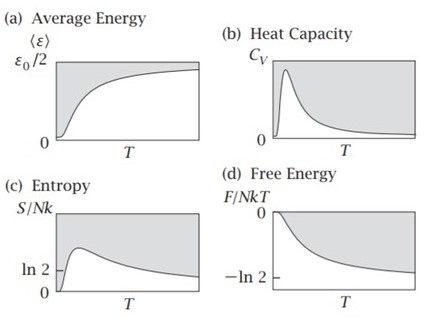
\includegraphics[width=8cm]{schottky}
	\centering
	\caption{}
	\label{fig:schottky}
\end{figure}
As shown in \Cref{fig:schottky} (b), there is a characteristic sharp peak in $C_V$ 
at intermediate temperatures, when the energy of the heat bath can most effectively 
excite the particles in the system. \\
Entropy is obtained by remembering
\begin{subequations}
\begin{align}
S&=k\ln Q+\frac{U}{T}\\
&=Nk\ln (1+e^{-\epsilon_0/kT})+\frac{N\epsilon_0e^{-\epsilon_0/kT}}{T(1+e^{-\epsilon_0/kT})}, 
\end{align}
\end{subequations}
and lastly, free energy:
\begin{equation}
A=-kT\ln Q=-NkT\ln(1+e^{-\epsilon_0/kT}).
\end{equation}
As $\epsilon_0\rightarrow\inf$, the excited states becomes inacessible and so 
$S\rightarrow0$ and $A\rightarrow0$. \\
As $\epsilon_0\rightarrow0$, two states are equally accessible and so 
$S\rightarrow Nk\ln 2$ and $A\rightarrow -NkT\ln 2$. 
\subsubsection{Curie's law of paramagnetism}
Paramagnetic materials are made up of atoms which have negligible dipole-dipole 
as compared to interaction with an applied field. 
Each atom has a magnetic dipole of magnitude $\mu_0>0$, and gives an energy of 
$-\mu_0B$ if the spin is aligned parallel to the field and $+\mu_0B$ if aligned 
antiparallel. Setting the ground state energy to $0$ we have our partition function: 
\begin{equation}
q=1+e^{-2\mu_0B/kT}.
\end{equation}
We would like to calculate the average magnetic moment. The probabilities are
\begin{equation}
p_1^*=\frac{1}{q}\ \ \ \text{and}\ \ \ p_2^*=\lf(\frac{1}{q} \rt)e^{-2\mu_0B/kT}.
\end{equation}
So the average dipole moment is calculated by
\begin{equation}
\lgl \mu\rgl=\mu_0p_1^*+(-\mu_0)p_2^*=\mu_0\frac{1-e^{-2\mu_0B/kT}}{1+e^{-2\mu_0B/kT}}=\mu_0\tanh\lf(\frac{\mu_0B}{kT}\rt).
\end{equation}
The Taylor series expansion gives 
\begin{equation}
\lgl \mu\rgl=\frac{\mu_0^2B}{kT}
\end{equation}
at small $\mu_0B/kT$, meaning high temperature and/or weak field. This is \textbf{Curie's law}. 
This explains the fact that cooling and high field strengths magnetise paramagnets effectively. 
\subsubsection{Modelling a protein loop}
test
\section{The statistical mechanics of simple gases}
\label{nststatmech}
\subsection{Molecular partition function}
\subsubsection{Translational partition function}
The quantum mechanical model of a particle in a potential well provides energy 
levels for such a particle, and the energies are given by
\begin{equation}
\epsilon_n=\frac{nh^2}{8mL^2}, 
\end{equation}
where $L$ is the length of the well. 
So the translational partition function is given by
\begin{equation}
q_{\text{trans}}=\sum^{\inf}_{n=1} e^{-\epsilon_n/kT}=\sum^{\inf}_{n=1} e^{-n^2h^2/(8mL^2kT)}.
\end{equation}
It is customary to define
\begin{defi}[Temperature of degrees of freedom]
Energies associated with degrees of freedom are usually divided by the 
Boltzmann factor and expressed in units of temperature. For example, the 
\textbf{translational temperature} is 
\begin{equation}
\theta_{\text{trans}}=\frac{h^2}{8mL^2k}, 
\end{equation}
such that partition function can be compactly written as 
\begin{equation}
q_{\text{trans}}=\sum^{\inf}_{n=1} e^{-n^2\theta/T},
\end{equation}
If the temperature of a degree of freedom is low, then the partition function 
can be \textit{approximated by an integral}. 
\end{defi}
Evidently, when $\theta/T\ll1$, the ability of the $n^2$ factor of bringing 
the magnitude of the exponential is limited, and a great many Boltzmann's factors 
will be evaluated at around $1$ until very large $n$ is reached. This means 
the partition function, and hence the number of effectively 
populated states is very large. This means we can approximate the sum as an integral: 
\begin{equation}
q_{\text{trans}}=\intinfp e^{(-h^2/8mL^2kT)n^2}\dif n=\lf(\frac{2\pi mkT}{h^2} \rt)^{1/2}L\equiv \frac{L}{\Lambda},
\end{equation}
where $\Lambda=(2\pi mkT/h^2)^{-1/2}$ is the \textbf{thermal wavelength}.
Now, for a 3D box of side lengths $a,b,c$, as the motion in each direction 
is assumed to be \textit{independent}, the wavefunction $\psi(x,y,z)$ can be 
separated into $\psi(x)\psi(y)\psi(z)$, and we can write
\begin{equation}
H\psi(x,y,z)=(H_x+H_y+H_z)\psi(x)\psi(y)\psi(z)=\epsilon_{n_x,n_y,n_z}\psi(x,y,z), 
\end{equation}
where 
\begin{equation}
H\equiv-\frac{\hbar^2}{2m}\lf(\diffp[2]{}{x}+\diffp[2]{}{y}+\diffp[2]{}{z} \rt)+\underbrace{V(x,y,z)}_{=0},
\end{equation}
and 
\begin{equation}
\ep_{n_x,n_y,n_z}=\frac{h^2}{8m}\lf(\frac{n_x^2}{a^2}+\frac{n_y^2}{b^2}+\frac{n_z^2}{c^2} \rt).
\end{equation}
As the energy can be separated into three dimensions (a direct result of the fact 
that their motions are independent, anyway), the Boltzmann factors are multiplied 
and hence can be independently evaluated and so the resulting partition functions 
are just the product of three one-dimentsional partition functions:
\begin{equation}
q_{\text{trans}}=q_xq_yq_z=\lf(\frac{2\pi mkT}{h^2} \rt)^{3/2}V\equiv\frac{V}{\Lambda^3}
\end{equation}
\begin{wex}
For temperature $T=273$K, and the volume $V=2.24\times10^{-2}\text{m}^3$ of one 
mole of gas at $p=1$atm, the translational partiton function is 
\begin{equation}
q_{\text{trans}}=\lf(\frac{2\pi mkT}{h^2} \rt)^{3/2}V.
\end{equation}
Substituting in mass for a single atom computed from molar mass, we have
\begin{equation}
q_{\text{trans}}\approx4.79\times10^{30}\ \text{states per atom}.
\end{equation}
\end{wex}
\subsubsection{Vibrational partition function}
The quantum mechanical harmonic oscillator model gives the energy of a harmonic 
oscillator as 
\begin{equation}
\ep_v=\hbar\omega\lf(v+\frac{1}{2} \rt),\ v=0,1,2,\cdots,
\end{equation}
where $\omega=\sqrt{k/\mu}$. We set the ground state energy 
$\ep_0=\hbar\omega/2$ to $0$, to get the partition function
\begin{equation}
q_{\text{vib}}=\sum^{\inf}_{v=0}e^{-\hbar\omega v/kT}\equiv1+x+x^2+\cdots=(1-x)^{-1}=\frac{1}{1-e^{-\hbar\omega/kT}}.
\end{equation}
We can use the Taylor series expansion because the vibrational temperture, given by
\begin{equation}
\theta_{\text{vib}}=\frac{\hbar\omega}{k}\approx10^3\ \text{K}
\end{equation}
is large enough to make sure that $|x|<1$, which is the condition of convergence for this Taylor series. 
\begin{wex}
Oxygen molecules have a vibrational wavenumber of $1580\ \text{cm}^{-1}$, so
\begin{equation}
\theta_{\text{vib}}=\frac{\hbar\omega}{k}\approx2274\ \text{K}.
\end{equation}
So the partition function at $T=300$ K is 
\begin{equation}
q_{\text{vib}}=\frac{1}{1-e^{-\theta/T}}\approx1.0005.
\end{equation}
So most oxygen molecules are in their ground vibrational states at this temperature. And even at $1000$ K, the partition function is only $1.11$. 
\end{wex}
For more complex molecules, as each vibrational mode has a separate set of vibrational wavefunctions and energies associated with them, the total partition function is just a product of the partition functions of each of the modes.
\subsubsection{Rotational partition function}
The rotational energy is given by 
\begin{equation}
\ep_{\ell}=\frac{\hbar^2}{2I}\ell(\ell+1),\ \ell=0,1,2,\cdots.
\end{equation}
There is a $2\ell+1$-fold degeneracy thanks to $m$, so the partition function is 
\begin{equation}
q_{\text{rot}}=\sum^{\inf}_{\ell=0} (2\ell+1)e^{-\ep_{\ell}/kT}\equiv \sum^{\inf}_{\ell=0} (2\ell+1)e^{-\theta_{\text{rot}}/T}.
\end{equation}
The rotational temperature is defined as 
\begin{equation}
\theta_{\text{rot}}\equiv\frac{\hbar^2}{2Ik}=\frac{\widetilde{B}}{\widetilde{k}}, 
\end{equation}
and is typically in the order of $10$ K, therefore, only in \textit{high 
temperature limit}, can we approximate the sum as an integral:
\begin{equation}
q_{\text{rot}}=\intinfp(2\ell+1)e^{-(\ell^2+\ell)\theta/T}\dif\ell=\frac{T}{\theta}.
\end{equation}
All very well, but we have to introduce a rotational symmetry factor $\sigma$: 
\begin{equation}
q_{\text{rot}}\equiv\frac{T}{\sigma\theta}.
\end{equation}
This factor accounts for the ways the molecule can indistinguishably overlap itself by rotation, for example, it takes on the values
\begin{singlespace}
\begin{equation}
\sigma=
\begin{cases}
1,\ &\text{heteronuclear diatomics}\\
2,\ &\text{homonuclear diatomics}\\
2,\ &\text{H$_2$O}\\
12,\ &\text{CH$_4$}\\
12,\ &\text{benzene}.
\end{cases}
\end{equation}
\end{singlespace}
These are essentially the number of all rotational classes in the point group the molecule belongs to, plus one (E operation).
For nonlinear molecules with three principal moments of inertia 
$I_a,I_b$ and $I_c$, the partition function is given, in the high temperature 
limit (\hl{proof needed}):
\begin{equation}
q_{\text{rot}}=\frac{(\pi I_aI_bI_c)^{1/2}}{\sigma}\lf(\frac{2kT}{\hbar^2} \rt)^{3/2}=\frac{\pi^{1/2}}{\sigma}\lf(\frac{T^3}{\theta_a\theta_b\theta_c} \rt)^{1/2},
\end{equation}
where the $a,b,c$ subscripts stand for the three axes of rotation.
However, for smaller molecules or lower temperatures, we cannot justifiably 
use the integral and must use the \textbf{Euler-Maclaurin formula} to 
approximate the sum. 
\begin{equation}
q_{\text{rot}}=\frac{T}{\theta}+\frac{1}{3}+\frac{1}{15}\frac{\theta}{T}+\frac{4}{315}\lf(\frac{\theta}{T}\rt)^2+\frac{1}{315}\lf(\frac{\theta}{T}\rt)^3+\cdots.
\end{equation}
\hl{how to get this from E-M formula?}
\subsubsection{Electronic partition function}
The electronic energy levels are usually large compared to $kT$ and as a result the excited levels do not contribute significantly to the overall partition function, however exceptions do exist, for example for Si(g)
\begin{center}
\begin{tabular}{r|c c c c c}
level & $^3$P$_0$ & $^3$P$_1$ & $^3$P$_2$ & $^1$D$_2$ & $^1$S$_0$\\
\hline
energy / cm$^{-1}$ & 0.0 & 76 & 222 & 6297 & 15390
\end{tabular}
\end{center}
The electronic partition function $q_{\text{el}}$ is given by
\begin{equation}
q_{\text{el}}=\sum_{i}g_i\exp(-\ep_i/kT),
\end{equation}
where $g_i=2J_i+1$, as the \emph{levels} ($J$) are degenerate (can take on different $M_J$, which are called states) in absense of external magnetic fields.
In this case $q_{\text{el}}$ is about $6.05$.\par
In \textbf{molecules}, the degeneracy is the product of the spin and spatial degeneracies, for exmample, $^3\Pi_u$ is $3\times 2=6$ degenerate.







\subsection{Interal energy and heat capacity}
An rule of thumb that works when $T\gg \theta$ is the equipartion principle.
\begin{thrm}[Equipartition principle]
The equipartition principle states that each `squared term' in the expression for the total energy\footnote{Quadratic in position or momentum variables} contributes $\frac{1}{2}RT$ per mole to the internal energy of the system.
\end{thrm}
To break it down, we look at the four contributors to internal energy.\par
\textbf{Translations}\\
Three squared terms, contribute to $3RT/2$ per mole.\par
\textbf{Rotations}\\
Three squared terms for \emph{non-linear} molecules, but two for \emph{linear} molecules. $3RT/2$ or $RT$ contribution respectively.\par
\textbf{Vibrations}\\
Vibrational energy is a sum of the kinetic energy and potential energy, therefore two squared terms are involved and contributes $RT$ to the internal energy.\par
\textbf{Electronic states}\\
It does not contain a squared term and falls outside the remit of the equipartition principle, but the ground state electronic energy is a significant contributor to internal energy \hl{update this}\par
As $C_v=\diffp U/T[V]$, we can easily see that the heat capacity will vary as follows
\begin{center}
\begin{tabular}{c|cc}
T / K & linear & non-linear\\
\hline
$T<\theta_{\text{rot}}$&$\frac{3}{2}R$&$\frac{3}{2}R$\\
$\theta_{\text{rot}}<T<\theta_{\text{vib}}$&$\frac{5}{2}R$&$3R$\\
$T>\theta_{\text{vib}}$&$\frac{7}{2}R$&$4R$\\
\end{tabular}
\end{center}
However the equipartition principle only works at large temperatures for each degree of freedom ($T\gg \theta$), and we outline the proof below
\textbf{Translational contribution}\\
Starting from
\begin{equation}
q_{\text{trans}}=\lf(\frac{2\pi mkT}{h^2} \rt)^{3/2}V\equiv\alpha T^{3/2},
\end{equation}
which \emph{already assumes the high temperature limit}, and 
\begin{equation}
U=NkT^2\diffp{\ln q}{T}[V]
\end{equation}
we arrive at
\begin{equation}
\begin{aligned}
U_{\text{trans}}&=NkT^2\diffp{\ln\alpha T^{3/2}}{T}[V]\\
&=NkT^2\diffp{\lf(\ln\alpha+\frac{3}{2}\ln T \rt)}{T}[V]\\
&=\frac{3}{2}NkT,
\end{aligned}
\end{equation}
and also that $C_{V,m,\text{trans}}=3R/2$.\par
\textbf{Rotational contribution}\\
Starting from
\begin{equation}
	q_{\text{rot}}=\frac{T}{\sigma\theta_{\text{rot}}},
\end{equation}
which \emph{also assumes the high temperature limit}, we get 
\begin{equation}
\begin{aligned}
	U_{\text{rot}}&=NkT^2\diffp{\ln{q_{\text{rot}}}}{T}[V]\\
	&=NkT^2\diffp{\ln{\alpha T}}{T}[V]\\
	&=NkT
\end{aligned}
\end{equation}
Which means a contribution of $R$ to the heat capacity.\\
\textbf{Vibrational contribution}\\
We start from
\begin{equation}
\label{qvib}
	q'_{\text{vib}}=\frac{1}{1-\exp(-\theta_{\text{vib}}/T)},
\end{equation}
which \emph{does not assume} high temperature limit, which we'll have to do later to recover the equipartition principle:
\begin{equation}
\label{uvib}
\begin{aligned}
	U'_{\text{vib}}&=NkT^2\diffp{\ln q'_{\text{vib}}}{T}[V]\\
	&\dots\\
	&=\frac{Nk\theta_{\text{vib}}}{\exp(\theta_{\text{vib}}/T)-1}
\end{aligned}
\end{equation}
$C_v$ is tedious to compute
\begin{equation}
	C_{v,\text{vib}}=\frac{Nk\theta_{\text{vib}}^2}{T^2}\frac{\exp(\theta_{\text{vib}}/T)}{[\exp(\theta_{\text{vib}}/T)-1]^2}.
\end{equation}
In the high temperature limit the Taylor expansion $e^x\approx 1+x+x^2/2+\dots $ applies,
\begin{equation}
\begin{aligned}
	&q'_{\text{vib}}\approx\frac{T}{\theta_{\text{vib}}}\\
	&U'_{\text{vib}}\approx NkT\\
	&C_v\approx Nk
\end{aligned}
\end{equation}


\subsection{Entropy}
We can write the total partition function for a system with $N$ particles as
\begin{equation}
\begin{aligned}
	Q&=Q_{\text{trans}}Q_{\text{rot}}Q_{\text{vib}}Q_{\text{el}}\\
	&=\frac{q^N_{\text{trans}}}{N!}q_{\text{rot}}^Nq_{\text{vib}}^Nq_{\text{el}}^N,
\end{aligned}
\end{equation}
where the indistinguishability of the particles only needs to be taken into account \emph{once}, and rotations etc. are treated as if the particles were in a crystal \ie distinguishable. This really only applies when the particles are \emph{weakly coupled}, which is not the case in liquids and solids. \par
With that out of the way, we recall that
\begin{equation}
	S=k\ln Q+\frac{U}{T}.
\end{equation}
\textbf{Translational entropy}\\
As
\begin{equation}
	q_{\text{trans}}=\lf(\frac{2\pi mkT}{h^2} \rt)^{3/2}V,
\end{equation}
we get
\begin{thrm}[The Sackur-Tetrode Equation]
The equation states
\begin{equation}
\begin{aligned}
		S_{\text{trans}}&=Nk\ln\lf[\lf(\frac{2\pi mkT}{h^2} \rt)^{3/2}V \rt]-Nk\ln N+Nk+\frac{3}{2}Nk\\
		&=Nk\lf\{\ln\lf[\lf(\frac{2\pi mkT}{h^2} \rt)^{3/2}V \rt]-\ln N+\frac{5}{2} \rt\}
\end{aligned}
\end{equation}
Further simplification under molar ideal gas conditions ($N=N_A,Nk=R,V=RT/p,m=M/N_A$)
\begin{equation}
\begin{aligned}
	S_{\text{trans},m}&=R\lf[\ln\lf(\frac{M^{3/2}T^{5/2}}{p} \rt) \rt]+20.723R\\
	&=\underbrace{R\ln V+\frac{3}{2}R\ln T}_{\text{classical}}+\underbrace{\frac{3}{2}R\ln M+18.605R}_{\text{non-classical}}
\end{aligned}
\end{equation}
\end{thrm}
\textbf{Rotational entropy}\\
\begin{equation}
	q_{\text{rot}}=\frac{T}{\sigma\theta_{\text{rot}}},
\end{equation}
so 
\begin{equation}
\begin{aligned}
	S_{\text{rot}}&=Nk\ln q_{\text{rot}}+\frac{U_{\text{rot}}}{T}\\
	&=Nk\lf[\ln\lf(\frac{T}{\sigma\theta_{\text{rot}}} \rt)+1 \rt]
\end{aligned}
\end{equation}
remembering the different values of $U_{\text{vib}}$ for linear and non-linear molecules, so for a non-linear molecule
\begin{equation}
	S_{\text{rot}}=Nk\lf[\ln\lf(\frac{T}{\sigma\theta_{\text{rot}}} \rt)+\frac{3}{2} \rt]
\end{equation}
\textbf{Vibrational entropy}\\
Not much can be done to simplify this, just substitute in \cref{qvib,uvib},
\begin{equation}
	S_{\text{vib}}=Nk\ln q'_{\text{vib}}+\frac{U'_{\text{vib}}}{T}
\end{equation}
Often it is the case that $q'_{\text{vib}}=1$ and so $U'_{\text{vib}}=0$, and there's no vibrational contribution, as to be expected when all particles are in ground state.\par
\textbf{Electronic entropy}
\begin{equation}
	S_{\text{el}}=Nk\ln q'_{\text{el}}+\frac{U'_{\text{el}}}{T}=Nk\ln g_0
\end{equation}
\textbf{Calorimetry}\\
To determine entropy experimentally, the following expression is used
\begin{equation}
\begin{aligned}
	S(T)&=\int_0^T\frac{C_p(T')}{T'}\dif T'+\sum_{\text{pc}}\frac{\Delta H_{\text{pc}}}{T_{\text{pc}}}\\
	&\approx\underbrace{\int_0^{T_0}\frac{aT'^3}{T'}\dif T'}_{\text{Debye law}}+\int_{T_0}^T\frac{C_p(T')}{T'}\dif T'+\sum_{\text{pc}}\frac{\Delta H_{\text{pc}}}{T_{\text{pc}}}
\end{aligned}
\end{equation}




\subsection{Nuclear spin partition function}
The nuclear spin quantum number $I$ can be an integer or a half-integer, and the projection onto $z$ axis is $M_I$, which run from $-I$ to $I$. In absence of external magnetic field these levels are degenerate.\par
In a diatomic molecule, in the weak-coupling approximation there are $(2I_1+1)\times(2I_2+1) $.\par
Now considering the example of $^1$H$^{19}$F, both have $I=1/2$ so we can denote the possible states as
\begin{equation}
\alpha(H)\alpha(F),\ \ \alpha(H)\beta(F),\ \ \beta(H)\alpha(F),\ \ \beta(H)\beta(F),\ \ 
\end{equation}
For a homonuclear diatomic though as the two nuclei are identical the situation is more complex, as for example $\alpha(1)\beta(2)$ produces $\alpha(2)\beta(1)$ is produced which is a completely different function which is unacceptable. We can follow the example of electron spins and product three triplet states, that \emph{doesn't} change sign under exchange of labels, and one singlet state, which \emph{does} change sign.\hl{incomplete}\par
\begin{thrm}[Number of sym and antisym nuclear spin states]
For a homonuclear diatomic, each atom with the nuclear spin $I$
\begin{equation}
\begin{aligned}
&\text{\# of symmetric states}=(2I+1)(I+1)\\
&\text{\# of antisymmetric states}=(2I+1)I
\end{aligned}
\end{equation}
\end{thrm}
\begin{proof}
There are $(2I+1)^2$ states in total, of which, $(2I+1)$ states have both the nuclei with the same spin \ie symmetric. The remaining states aren't simply symmetric or antisymmetric as nuclear exchange produces entirely different states. Therefore two linear combinations can be formed between two permuted states\footnote{This means $\alpha(1)\gamma(2) $ and $\gamma(1)\alpha(2) $, or $\delta(1)\beta(2) $ and $\beta(1)\delta(2)$, where the greek letters denote different spins.} to produce symmetric and antisymmetric wavefunctions. This means half of the remaining states will be symmetric and half antisymmetric. This brings the total to
\begin{equation}
\begin{aligned}
&\text{\# of symmetric states}=(2I+1)+(2I+1)I=(2I+1)(I+1)\\
&\text{\# of antisymmetric states}=(2I+1)I
\end{aligned}
\end{equation}
\end{proof}
\subsubsection{Nuclear exchange}
Exchange of nuclear labels must be done in way that does not affect other wavefunctions, so a simple 180$^{\circ}$ rotation ($C_2$) won't do. The following operations are needed
\begin{enumerate}
  \item $C_2$, but electrons around the nuclei are moved as well, nuclear spin states are not affected.
  \item $i_{\text{elec}}$ Invert just the electrons through the centre of inversion.
  \item $\sigma_{\text{elec}} $ Reflect just the electrons in a plane containing the internuclear axis.
  \item $\rho_{\text{nuc}}$, permutes (flips) the nuclear spin states.
\end{enumerate}
These are going to have the following effects on the overall wavefunction
\begin{enumerate}
  \item $C_2$: $\psi_{\text{elec}}$ and $\psi_{\text{vib}}$ are unaffected, however $\psi_{\text{rot}}$ will be affected in the same way as the spherical harmonics, which means even $J$ is unchanged, and odd $J$ changes sign
  \item $i_{\text{elec}}$: this depends on the inversion symmetry ($g/u$) of the molecular term symbol, $g$ doesn't change sign and $u$ does.
  \item $\sigma_{\text{elec}} $: this depends on the reflection symmetry ($\pm$), $+$ doesn't change sign and $-$ does.
  \item $\rho_{\text{nuc}}$: symmetric states don't change sign and asymmetric states do.
 \end{enumerate}
\subsubsection{Consequences on spectroscopy}
\label{nucspinspec}
We will look at the consequence of this for a few examples.\par
\textbf{$^1$H$_2$}\\
We go through a checklist
\begin{enumerate}
  \item The ground state is $^1\Sigma_g^+$
  \begin{enumerate}
  \item The overall wavefunction is symmetric to $\sigma_{\text{elec}}$.
  \item The overall wavefunction is also symmetric to $i_{\text{elec}}$.
\end{enumerate}
  \item $^1$H has $I=1/2$
\begin{enumerate}
  \item It is a fermion, the overall wavefunction must be antisymmetric wrt. nuclear exchange.
  \item There are 3 symmetric nuclear spin states and 1 antisymmetric nuclear spin states.
\end{enumerate}
\end{enumerate}
We can now generate the following table
\begin{center}
\begin{tabular}{cc|cccc|c}
\hline
rotational & nuclear spin & $C_2$ & $i_{\text{elec}}$ & $\sigma_{\text{elec}}$ & $\rho_{\text{nuc}}$ & overall\\
\hline
even J & sym & $+$ & $+$ & $+$ & $+$(3) & $+$(forbidden)\\
even J & antisym & $+$ & $+$ & $+$ & $-$(1) & $-$(permitted)\\
odd J & sym & $-$ & $+$ & $+$ & $+$(3) & $-$(permitted)\\
odd J & antisym & $-$ & $+$ & $+$ & $-$(1) & $+$(forbidden)\\
\hline
\end{tabular}
\end{center}
This means that rotational states with odd $J$ values have three times the statistical weight than those with even values. This will result in the a Raman spectrum with alternately high and low peaks: 
\begin{equation}
\begin{aligned}
I_{\text{odd }J}&\propto 3\times(2J+1)\exp\lf[\frac{-BJ(J+1)}{kT} \rt]\\
I_{\text{even }J}&\propto 1\times(2J+1)\exp\lf[\frac{-BJ(J+1)}{kT} \rt]
\end{aligned}
\end{equation}
where the extra factor in front is the ratio between the numbers of \emph{ortho} (sym) and \emph{para} (antisym) H$_2$ molecules. The high temperature equilibrium is intuitively $3:1$, but we shall prove it in the next section.\par
\textbf{$^{14}$N$_2$}
\begin{enumerate}
  \item The ground state is $^1\Sigma_g^+$
  \begin{enumerate}
  \item The overall wavefunction is symmetric to $\sigma_{\text{elec}}$.
  \item The overall wavefunction is also symmetric to $i_{\text{elec}}$.
\end{enumerate}
\item $^{14}N$ has $I=1$
\begin{enumerate}
  \item It is a boson, the overall wavefunction must be antisymmetric wrt. nuclear exchange.
  \item There are 6 symmetric nuclear spin states and 3 antisymmetric nuclear spin states.
\end{enumerate}
\end{enumerate}
The table is 
\begin{center}
\begin{tabular}{cc|cccc|c}
\hline
rotational & nucealr spin & $C_2$ & $i_{\text{elec}}$ & $\sigma_{\text{elec}}$ & $\rho_{\text{nuc}}$ & overall\\
\hline
even J & sym & $+$ & $+$ & $+$ & $+$(6) & $+$(permitted)\\
even J & antisym & $+$ & $+$ & $+$ & $-$(3) & $-$(forbidden)\\
odd J & sym & $-$ & $+$ & $+$ & $+$(6) & $-$(forbidden)\\
odd J & antisym & $-$ & $+$ & $+$ & $-$(3) & $+$(permitted)\\
\hline
\end{tabular}
\end{center}
The ratio of odd and even $J$ states are now 1:2 (ortho:para nitrogen).\par
\textbf{$^{16}$O$_2$} (spin zero)
\begin{enumerate}
  \item The ground state is $^3\Sigma_g^-$
  \begin{enumerate}
  \item The overall wavefunction is antisymmetric to $\sigma_{\text{elec}}$.
  \item The overall wavefunction is symmetric to $i_{\text{elec}}$.
\end{enumerate}
\item $^{16}O$ has $I=0$
\begin{enumerate}
  \item It is a boson, the overall wavefunction must be antisymmetric wrt. nuclear exchange.
  \item There are 1 symmetric nuclear spin states and 0 antisymmetric nuclear spin states.
\end{enumerate}
\end{enumerate}
The table is thus
\begin{center}
\begin{tabular}{cc|cccc|c}
\hline
rotational & nucealr spin & $C_2$ & $i_{\text{elec}}$ & $\sigma_{\text{elec}}$ & $\rho_{\text{nuc}}$ & overall\\
\hline
even J & sym & $+$ & $+$ & $-$ & $+$(1) & $-$(forbidden)\\
odd J & sym & $-$ & $+$ & $-$ & $+$(1) & $+$(permitted)\\
\hline
\end{tabular}
\end{center}
$^{16}$O$_2$ can only exist in odd $J$ states, which clearly will have an effect on the Raman spectrum (10$\widetilde{B}_0$, 8$\widetilde{B}_0$, 8$\widetilde{B}_0$\dots)\par
\textbf{$^{12}$C$^{16}$O$_2$}\\
C lies in the centre of symmetry so is not affected by nuclear exchange, so we just need to consider the two oxygen atoms.
\begin{enumerate}
  \item The ground state is $^1\Sigma_g^+$
  \begin{enumerate}
  \item The overall wavefunction is symmetryic to $\sigma_{\text{elec}}$.
  \item The overall wavefunction is antisymmetric to $i_{\text{elec}}$.
\end{enumerate}
\item $^{16}O$ has $I=0$ (same as above)
\begin{enumerate}
  \item It is a boson, the overall wavefunction must be antisymmetric wrt. nuclear exchange.
  \item There are 1 symmetric nuclear spin states and 0 antisymmetric nuclear spin states.
\end{enumerate}
\end{enumerate}
Therefore we have
\begin{center}
\begin{tabular}{cc|cccc|c}
\hline
rotational & nucealr spin & $C_2$ & $i_{\text{elec}}$ & $\sigma_{\text{elec}}$ & $\rho_{\text{nuc}}$ & overall\\
\hline
even J & sym & $+$ & $+$ & $+$ & $+$(1) & $+$(permitted)\\
odd J & sym & $-$ & $+$ & $+$ & $+$(1) & $-$(forbidden)\\
\hline
\end{tabular}
\end{center}
So this is clearly the opposite case as the dioxygen, in the \emph{pure rotational Raman} spectrum, only even $S$ lines are seen, with spacings of 6$\widetilde{B}_0$, 8$\widetilde{B}_0$, 8$\widetilde{B}_0$\dots\par
The effect on the \emph{IR spectrum} however is subtly different, as the selection rule of IR spectrum is $\Delta J=\pm1$, we might expect the $PR$ rotational fine structure to not come up at all, but this is not the case. Thinking carefully, we have been working on the assumption that all the rotational states belong to the ground vibrational state, as is the case for \emph{pure rotational Raman}, so it has been implicit that there's a coloumn for `vibrational', under which it has always been symmetrical\footnote{This is because all vibrational ground states belong to the totally symemtric irreducible representation.}, and that will be absorbed into the the sign/parity under $C_2$. So now, with the IR-active normal mode, we have alternately symmetric and antisymmetric vibrational wavefunctions, and so we can generate 
\begin{center}
\begin{tabular}{ccc|cccc|c}
\hline
vibrational & rotational & nucealr spin & $C_2$ & $i_{\text{elec}}$ & $\sigma_{\text{elec}}$ & $\rho_{\text{nuc}}$ & overall\\
\hline
\multicolumn{8}{c}{$v=0$}\\
\hline
sym & even J & sym & $+$ & $+$ & $+$ & $+$(1) & $+$(permitted)\\
sym & odd J & sym & $-$ & $+$ & $+$ & $+$(1) & $-$(forbidden)\\
\hline
\multicolumn{8}{c}{$v=1$}\\
\hline
antisym & even J & sym & $-$ & $+$ & $+$ & $+$(1) & $-$(forbidden)\\
antisym & odd J & sym & $+$ & $+$ & $+$ & $+$(1) & $+$(permitted)\\
\hline
\end{tabular}
\end{center}
and we can clearly see that now transitions between even and odd $J$ are allowed, \emph{given that} the vibrational levels also change in parity\footnote{This is true as long as the normal mode belongs to a symmetry species that is \emph{not} invariant under $C_2$.}, the \emph{rotational fine structure} will appear `normal'. The same argument applies for the Raman-active modes, however the rotation fine structures there are less resolved.

\subsubsection{Consequences on rotational partition function}
The symmetry factor $\sigma_{\text{rot}}$ arises from the fact that \emph{nuclear spin and rotational wavefunctions are coupled} in homonuclear diatomics (and molecules with an array of other symmetries, but it's too complicated to go into those), so we have to evaluate the two partition functions together. For heteronuclear diatomics they are uncoupled and they can be simply computed separately:
\begin{equation}
  q_{\text{NS}}q_{\text{rot}}=(2I_1+1)(2I_2+1)\sum_J(2J+1)\exp\lf(\frac{-BJ(J+1)}{kT} \rt)
\end{equation}
But in a homonuclear diatomic, we have to write
\begin{equation}
\begin{aligned}
  q_{\text{NS}}q_{\text{rot}}=&g_{\text{NS, even}}\sum_{\text{even }J}(2J+1)\exp\lf(\frac{-BJ(J+1)}{kT} \rt)\\
&+g_{\text{NS, odd}}\sum_{\text{odd }J}(2J+1)\exp\lf(\frac{-BJ(J+1)}{kT} \rt)
\end{aligned}
\end{equation}
in the limit of $kT\gg B$, there are many terms contributing to the sum, and the odd and even sums are roughly equal to if all $J$ were to be summed up, which would have given $kT/B$, so the odd and even sums here are both equal to $kT/2B$, and the product is
\begin{equation}
  q_{\text{NS}}q_{\text{rot}}=(g_{\text{NS, even}}+g_{\text{NS, odd}})\frac{kT}{2B}=g_{\text{NS}}\frac{kT}{2B}
\end{equation}
which effectively has given us a factor of $2$ in the denominator, which is the origin of the symmetry factor $\sigma_{\text{rot}}$.

\section{Chemical equilibrium}
\subsection{Preliminaries}
\subsubsection{Chemical potential}
Referring to \cref{eulergibbs}, we can write the Gibbs free energy as 
\begin{equation}
  G=\sum\mu_i N_i
\end{equation}
This applies for all homogeneous mixtures. From the master equation we also have
\begin{equation}
  \mu_i=\diffp{G}{n_i}[p,T,n_j]
\end{equation}
at constant $p$ and $T$ we can write
\begin{equation}
  \dif G=\sum_i\dif n_i\mu_i
\end{equation}
Consider the following chemical reaction
\begin{equation}
  \ch{$\nu$_AA + $\nu$_BB <=> $\nu$_MM + $\nu$_NN}
\end{equation}
we can write the change in Gibbs energy when $\dif z$ amount of reaction takes place:
\begin{equation}
  \dif G=+\nu_M\dif z\mu_M+\nu_N\dif z\mu_N-\nu_A\dif z\mu_A-\nu_B\dif z\mu_B
\end{equation}
which can be rearranged to give
\begin{equation}
  \diff Gz=+\nu_M\mu_M+\nu_N\mu_N-\nu_A\mu_A-\nu_B\mu_B
\end{equation}
And at equilibrium, we have $\diff G/z=0$, so
\begin{equation}
  0=+\nu_M\mu^{\text{eq}}_M+\nu_N\mu^{\text{eq}}_N-\nu_A\mu^{\text{eq}}_A-\nu_B\mu^{\text{eq}}_B
\end{equation}
Switching to working with Helmholtz energy, we have
\begin{equation}
  \mu_i=\diffp{A}{N_i}[V,T,N_j]
\end{equation}
which can be computed by using 
\begin{equation}
  A=-NkT\ln q+kT(N\ln N-N)
\end{equation}
so, assuming the species are non-interacting, we can write
\begin{equation}
  \mu_i=-kT\ln\frac{q_i}{N_i}
\end{equation}
\subsubsection{Choice of energy zero}
\begin{center}
  \begin{tabular}{c|c}
  Energy & Zero\\
  \hline
  Translational & Already zero\\
  Rotational & Already zero\\
  Vibrational & Bottom of well\\
  Electronic & Dissociated atoms
  \end{tabular}
\end{center}
So we can choose to write the Helmholtz energy as
\begin{equation}
  A=-NkT\ln q+kT(N\ln N-N)+N\ep^0
\end{equation}
where 
\begin{equation}
  q=q_{\text{trans}}q_{\text{rot}}q_{\text{vib}}q_{\text{el}}
\end{equation}
and $q_{\text{vib}}$ refers to bottom of well and $q_{\text{el}}$ takes electronic ground state as energy, zero, and the referral to dissociated atoms is done in the \emph{offset term} $N\ep^0$.\footnote{This is justified as $N\ln\sum_ig_i\exp(-\ep^i/kT)=N\ep^0+N\ln\sum_ig_i\exp(-(\ep^i-\ep^0)/kT)$.} For species $i$ in an \emph{ideal} mixture this is then
\begin{equation}
  \mu_i=-kT\ln\frac{q_i}{N_i}+\ep^{0,i}
\end{equation}
\subsection{Equilibrium constants}
\subsubsection{Calculation of \texorpdfstring{$K_c$}{Kc}}
Considering the same chemical reaction 
\begin{equation}
  \ch{$\nu$_AA + $\nu$_BB <=> $\nu$_MM + $\nu$_NN}
\end{equation}
with
\begin{equation}
\label{eqmchem}
  0=+\nu_M\mu^{\text{eq}}_M+\nu_N\mu^{\text{eq}}_N-\nu_A\mu^{\text{eq}}_A-\nu_B\mu^{\text{eq}}_B
\end{equation}
where we will omit the `eq' subscript and take it as implicit from now. \par
Only $q_{\text{trans}}$ contains a volume term, so we can write
\begin{equation}
  q=fV
\end{equation}
where
\begin{equation}
  f=\frac{q_{\text{trans}}}{V}q_{\text{rot}}q_{\text{vib}}q_{\text{el}}=\lf(\frac{2\pi mkT}{h^2} \rt)^{3/2}q_{\text{rot}}q_{\text{vib}}q_{\text{el}}
\end{equation}
so
\begin{equation}
  \mu_i=-kT\ln\frac{f_iV}{N_i}+\ep^{0,i}=-kT\ln\frac{f_i}{c_i}+\ep^{0,i}
\end{equation}
Clearly, sticking to the SI units, the units of $c_i$ is molecules / m$^3$. Substituting this into \cref{eqmchem}, we get
\begin{equation}
\begin{aligned}
  0=&+\nu_M\lf(-kT\ln\frac{f_M}{c_M}+\ep^{0,M} \rt)+\nu_N\lf(-kT\ln\frac{f_N}{c_N}+\ep^{0,N} \rt)\\
  &-\nu_A\lf(-kT\ln\frac{f_A}{c_A}+\ep^{0,A} \rt)-\nu_B\lf(-kT\ln\frac{f_B}{c_B}+\ep^{0,B} \rt)
\end{aligned}
\end{equation}
Rearrangement gives
\begin{equation}
  kT\ln\frac{c_M^{\nu_M}c_N^{\nu_N}}{c_A^{\nu_A}c_B^{\nu_B}}=kT\ln\frac{f_M^{\nu_M}f_N^{\nu_N}}{f_A^{\nu_A}f_B^{\nu_B}}-\Delta\ep_0
\end{equation}
where $\Delta\ep_0$ is the energy of products minus reactants. Cleaning up further we have
\begin{equation}
  K_c'=\frac{c_M^{\nu_M}c_N^{\nu_N}}{c_A^{\nu_A}c_B^{\nu_B}}=\frac{f_M^{\nu_M}f_N^{\nu_N}}{f_A^{\nu_A}f_B^{\nu_B}}\exp(-\Delta\ep_0/kT)
\end{equation}
Recalling the proper thermodynamic $K_c$ is
\begin{equation}
  K_c=\frac{\alpha_M^{\nu_M}\alpha_N^{\nu_N}}{\alpha_A^{\nu_A}\alpha_B^{\nu_B}}
\end{equation}
$\alpha_i$ in an \emph{ideal} aqueous solution is
\begin{equation}
  \alpha_i=\frac{c_i}{c^{\circ}}
\end{equation}
So we can obtain the `actual' $K_c$ easily
\begin{equation}
  K_c=K_c'\lf(\frac{1}{c^{\circ}}\rt)^{\Delta\nu}
\end{equation}
The reference state $c^{\circ}$ is \emph{always} given in units of molecules / m$^3$, as this expression arise from statistical mechanics. So for a final $K_c$ referred to the usual standard state of 1 mol / dm$^3$, $c^{\circ}$ is chosen to be $1000N_A$.\par
So we arrive at
\begin{thrm}[Expression of $K_c$]
\label{statmechkc}
The full expression of $K_c$ is
\begin{equation}
  K_c=\frac{f_M^{\nu_M}f_N^{\nu_N}}{f_A^{\nu_A}f_B^{\nu_B}}\lf(\frac{1}{c^{\circ}}\rt)^{\Delta\nu}\exp(-\Delta\ep_0/kT)
\end{equation}
where $\Delta\ep_0$ is the energy change, at absoulte zero, per molecule, and $K_c$ is dimensionless.
\end{thrm}
\paragraph{Interpretation}
Considering a simple reaction
\begin{equation*}
  \ch{A <=> M}
\end{equation*}
We can write the $K_c$ as
\begin{equation}
  K_c=\frac{f_M(T)}{f_A(T)}\exp(-\Delta\ep_0/kT)
\end{equation}
where the temperature dependence is made explicit, at low temperatures, only ground states are accessible and the exponential term is large, so it predominates, the equilibirum constant is less than one. At high temperatures, the ratio $f_M/f_A$ depends on the density of states of the two species - if the M states are denser than the A states, the ratio predominates the exponential, and the reaction will be entropically driven to the right.
\subsubsection{Calculation of \texorpdfstring{$K_p$}{Kp}}
If we start with \cref{stdgibbsp}, writing 
\begin{equation}
\label{kp1}
  \Delta_rG^{\circ}=\nu_M\mu^{\circ}_M+\nu_N\mu^{\circ}_N-\nu_A\mu^{\circ}_A-\nu_B\mu^{\circ}_B
\end{equation}
where
\begin{equation}
\label{kp2}
  \mu_i^{\circ}=N_A\lf(-kT\ln\frac{q_i^{\circ}}{N_A}+\ep^{0,i} \rt)=-RT\ln\frac{q_i^{\circ}}{N_A}+\ep_m^{0,i}
\end{equation}
in which $q^{\circ}$ is the molar partition function in the standard state, which only concerns the volume, which will be the standard molar volume $V_m^{\circ}$\footnote{Remember that temperature is not part of the standard state, so temperature is still an independent variable.}, so we can write
\begin{equation}
\label{kp3}
\begin{aligned}
  q^{\circ}&=q_{\text{trans}}q_{\text{rot}}q_{\text{vib}}q_{\text{el}}\\
  &=\lf(\frac{2\pi mkT}{h^2} \rt)^{3/2}V_m^{\circ}q_{\text{rot}}q_{\text{vib}}q_{\text{el}}\\
  &=\lf(\frac{2\pi mkT}{h^2} \rt)^{3/2}\lf(\frac{RT}{p^{\circ}} \rt)q_{\text{rot}}q_{\text{vib}}q_{\text{el}}
\end{aligned}
\end{equation}
Substituting \cref{kp2} into \cref{kp1} we can have the following result
\begin{thrm}[Expression of $K_p$]
The equilibrium constant is given by
\begin{equation}
  K_p=\frac{(q^{\circ}_M)^{\nu_M}(q^{\circ}_N)^{\nu_N}}{(q^{\circ}_A)^{\nu_A}(q^{\circ}_B)^{\nu_B}}(N_A)^{-\Delta\nu}\exp\lf(-\frac{\Delta\ep_0}{kT} \rt)
\end{equation}
\end{thrm}
\subsection{Examples}
\subsubsection{Dissociation of a diatomic}
We want to calculate the $K_c$ of the following reaction
\begin{equation*}
  \ch{A_2 <=> 2 A}
\end{equation*}
We note that $\Delta\nu=1$, $\Delta\ep_0=D_e$, so
\begin{equation}
  K_c=\frac{f_A^2}{f_{A_2}}\frac{1}{c^{\circ}}\exp(-D_e/kT)
\end{equation}
The key thing to remember is just that $\sigma$ for $A_2$ is 2, and also that the electronic ground state degeneracies might differ.\par
Different isotopes can also give different $K_c$, now consider the two reactions
\begin{equation}
\begin{aligned}
\ch{H + D &-> HD}\\
\ch{H + H &-> H2}
\end{aligned}
\end{equation}
At first sight we don't expect the rate constants to be different, but they the first is two times bigger than the second, even after taking the difference in masses into account. The reason will be clear if we write out the expressions for the equilibrium constants:
\begin{equation}
\begin{aligned}
    &K_c=\frac{f_{\ch{HD}}}{f_{\ch{H}}f_{\ch{D}}}\lf(\frac{1}{c^{\circ}}\rt)^{-1}\exp(-\Delta\ep_0/kT)\\
    &K_c=\frac{f_{\ch{H2}}}{f^2_{\ch{H}}}\lf(\frac{1}{c^{\circ}}\rt)^{-1}\exp(-\Delta\ep_0/kT)
\end{aligned}
\end{equation}
Just focussing on the electronic and rotational parts of the wavefunction, as the vibrational and translational (difference in masses already accounted for) are the same, we can write
\begin{equation}
  K_c\propto\frac{g_{0,\ch{AB}}}{g_{0,\ch{A}}g_{0,\ch{B}}}\frac{1}{\sigma}
\end{equation}
For the first reaction, the first bit will return $\frac{1}{4}$, and this can be interpreted as the fact that only when spins of the two atoms are antiparallel (singlet) can the two atoms form a bond, which means only one in four spin configurations can lead to reaction, the other three being the triplet state.\par
For the second reaction, the first bit is also $\frac{1}{4}$, but the second is $\frac{1}{2}$, which can be interpreted as that half of all rotational-nuclear states are disallowed, as the two are coupled in a homonuclear diatomic, see \cref{nucspinspec}.

\subsubsection{Ionisation of atoms}
The equation is 
\begin{equation*}
  \ch{M(g) <=> M^+(g) + e- (g)}
\end{equation*}
We again note that $\Delta\nu=1$, $\Delta\ep_0=E_1$, the ionisation energy (per molecule of course, if per mole divide by $RT$ instead), so
\begin{equation}
  K_c=\frac{f_ef_{M^+}}{f_M}\frac{1}{c^{\circ}}\exp(-E_1/kT)
\end{equation}
The masses of \ch{M} and \ch{M+} cancel out, electron has $g_0=2$ as it has spin one half, so we can write
\begin{equation}
  K_c=\lf(\frac{2\pi m_ekT}{h^2} \rt)^{3/2}\frac{2g_{0,\ch{M+}}}{g_{0,\ch{M}}}\frac{1}{c^{\circ}}\exp{-E_1/kT}
\end{equation}
cleaning up we have the 
\begin{thrm}[The Saha equation]
The Saha equation is used in the spectral classification of stars, which can be treated as gases at high enough temperatures, and it's given by
\begin{equation}
  K_c=\frac{2}{\Lambda^3}\frac{g_+}{g_0}\exp(-E_1/kT)
\end{equation}
where 
\begin{equation}
  \Lambda=\sqrt{\frac{h^2}{2\pi m_ekT}}
\end{equation}
is the thermal wavelength of an electron, and $g_+$ is the ground state degeneracy of the ion and $g_0$ of the atom.
\end{thrm}

\subsubsection{Adsorption of a gas}
The general equation for adsorption is
\begin{equation*}
  \ch{A_{g} + S <=>[ $k_a$ ][ $k_d$ ] A_{ad} }
\end{equation*}
where \ch{A_g} is the adsorbate molecule, \ch{S} are sites on a surface, and \ch{A_{ad}} is the adsorbed molecule
\begin{thrm}[Langmuir isotherm]
The Langmuir isotherm governs the proportion of gas that's adsorbed at equilibrium and it's given by
\begin{equation}
  \theta=\frac{K_{\text{ads}}p}{1+K_{\text{ads}}p}
\end{equation}
\end{thrm}
\begin{proof}
  The rate of adsorption is proportional to the amount of available sites and the gas pressure:
  \begin{equation}
    R_{\text{adsorption}}=k'_a[\ch{S}][\ch{A_g}] =k_a\times(M-N)\times p
  \end{equation}
  where $k_a$ absorbs an arbitrary conversion factor from $[\ch{A_g}]$ to $p$.\par
  The rate of desorption is only proportional to the amount of occupied sites:
  \begin{equation}
    R_{\text{desorption}}=k_d'[\ch{A_{ad}}] =k_d\times N
  \end{equation}
  At equilibrium the two must be equal, so we can write
  \begin{equation}
    K_{\text{ads}}=\frac{k_a}{k_d}=\frac{N}{M-N}\frac{1}{p}=\frac{\theta}{1-\theta}\frac{1}{p}
  \end{equation}
  Which rearranges easily to give the Langmuir isotherm.
\end{proof}
\paragraph{Monatomic gas}
Now we wish to find an expression of $K_{\text{ads}}$ for the simplest case of a monatomic gas. We note that at equilibirum
\begin{equation}
  \mu(\text{ads})=\mu(\text{g})
\end{equation}
for the free adsorbate gas, we further assume that it's a monatomic gas, so
\begin{equation}
  \mu(\text{ads})=kT\ln\lf(\frac{q_{\text{trans}}}{N_{\text{gas}}} \rt)+\ep^{0}_{\text{free}}=-kT\ln\lf(\frac{kT}{p\Lambda^3} \rt)+\ep^0_{\text{free}}
\end{equation}\footnote{We have ignored the electronic partition functions here as they cancel out. They should generally be included.}
For the adsorbed atoms it's less straightforward, we first write the Helmholtz energy for the system as
\begin{equation}
  A=-kT\ln Q_N
\end{equation}
We then note that 
\begin{equation}
  Q_N=\sum_m\exp(-E_m/kT)
\end{equation}
and we assume that all arrangements of the atoms have the same energy \ie the sites are equivalent and non-interacting, so $Q_N$ is simply the number of ways to arrange $N$ atoms in $M$ sites where $M\gg N$:
\begin{equation}
  Q_N=\frac{M!}{N!(M-N)!}
\end{equation}
so
\begin{equation}
  A=kT[-M\ln M+N\ln N+(M-N)\ln(M-N)]
\end{equation}
and by definition
\begin{equation}
  \mu=\diffp AN[T,V]
\end{equation}
with the offset correction this computes to
\begin{equation}
  \mu(\text{ads})=kT\ln\lf(\frac{N}{M-N} \rt)+\ep^0_{\text{ads}}=kT\ln\lf(\frac{\theta}{1-\theta} \rt)+\ep^0_{\text{ads}}
\end{equation}
equating the two chemical potentials we have
\begin{equation}
  -kT\ln\lf(\frac{kT}{p\Lambda^3} \rt)+\ep^0_{\text{free}}=kT\ln\lf(\frac{\theta}{1-\theta} \rt)+\ep^0_{\text{ads}}
\end{equation}
which rearranges to
\begin{equation}
  \lf(\frac{\theta}{1-\theta} \rt)\frac{1}{p}=\frac{\Lambda^3}{kT}\exp\lf(\frac{-\Delta\ep^0}{kT} \rt)
\end{equation}
the LHS of the equation can be identified as $K_{\text{ads}}$, the expression for $\theta$ is then
\begin{equation}
  \theta=\frac{bp}{1+bp}
\end{equation}
where
\begin{equation}
  b=\frac{\Lambda^3}{kT}\exp\lf(\frac{-\Delta\ep^0}{kT} \rt)
\end{equation}
and
\begin{equation}
  \Lambda=\sqrt{\frac{h^2}{2\pi mkT}}
\end{equation}
\begin{thrm}[Expression of $K_{\text{ads}}$ for monatomic gas]
The adsorption equilibrium constant of a monatomic gas is given by
\begin{equation}
  K_{\text{ads}}=\frac{\Lambda^3}{kT}\exp(-\Delta\ep^0/kT )
\end{equation}
with the fraction of adsorbed atoms given by
\begin{equation}
  \theta=\frac{K_{\text{ads}}p}{1+K_{\text{ads}}p}
\end{equation}
\end{thrm}
\paragraph{Non-dissociative molecular adsorption}
This is almost exactly the same as the monatomic gas except now there are internal contributors of partition function:
\begin{equation}
  Q_{N,\text{ads}}=q_{\text{ads}}^N\frac{M!}{N!(M-N)!}
\end{equation}
where $q_{\text{ads}}=q_{\text{vib}}q_{\text{rot}}$ is the internal degrees of freedom. We've omitted the electronic partition functions again as they'll cancel out. The chemical potential is thus
\begin{equation}
  \mu(\text{ads})=-kT\ln q_{\text{ads}}+kT\ln\lf(\frac{\theta}{1-\theta} \rt)+\ep^0_{\text{ads}}
\end{equation}
where $\theta=N/M$, the \emph{coverage factor}.\par
For the free gas,
\begin{equation}
  \mu(\text{g})=-kT\ln\lf(\frac{q}{N} \rt)+\ep^0_{\text{free}}=-kT\ln\lf(\frac{kT}{p\Lambda^3}q_{\text{free}} \rt)+\ep^0_{\text{free}}
\end{equation}
where again $q_{\text{free}}$ is the internal degrees of freedom, omitting electronic. We go through the same steps to obtain
\begin{thrm}[Non-dissociative adsorption]
The equilibrium constant is given as
\begin{equation}
  K_{\text{ads}}=\frac{q_{\text{ads}}}{q_{\text{free}}}\frac{\Lambda^3}{kT}\exp(-\Delta\ep^0/kT )
\end{equation}
\end{thrm}
\paragraph{Dissociative molecular adsorption}
Now we consider the reaction
\begin{equation*}
  \ch{H2 (g) + S <=> 2 H(ads)}
\end{equation*}
For $N$ \ch{H2} gas molecules, there are $M$ sites for \ch{H} \emph{atoms}, the number of ways to fit the molecules onto the sites is, in the limit that $M\gg N$,
\begin{equation}
 ^{M/2}C_N=\frac{(M/2)!}{N!(M/2-N)!}
\end{equation}
where the the hydrogen molecules have effective access to $M/2$ sites. The partition function of the system is then
\begin{equation}
  Q_N=\frac{(M/2)!}{N!(M/2-N)!}q_{\ch{H}}^{2N}
\end{equation}
where all the hydrogen atoms are distinguishable, and the partition function just includes the electronic partition function. So the chemical potential is
\begin{equation}
  \mu(\text{ads})=-2kT\ln q_{\text{H}}+kT\ln\lf(\frac{\theta}{1-\theta} \rt)+\ep^0_{\text{ads}}
\end{equation}
For the free gas it is the same as before,
\begin{equation}
  \mu(\text{g})=-kT\ln\lf(\frac{kT}{p\Lambda^3}q_{\ch{H2}} \rt)+\ep^0_{\text{free}}
\end{equation}
At equilibrium,
\begin{equation}
  \mu(\text{g})=2\mu(\text{ads})
\end{equation}
and so we can write
\begin{equation}
\begin{aligned}
  -kT\ln\lf(\frac{kT}{p\Lambda^3}q_{\ch{H2}} \rt)+\ep^0_{\text{free}}&=2\lf[ -2kT\ln q_{\text{H}}+kT\ln\lf(\frac{\theta}{1-\theta} \rt)+\ep^0_{\text{ads}}\rt]\\
-\ln\lf(\frac{kT}{p\Lambda^3}q_{\ch{H2}} \rt)=-2\ln q_{\ch{H}}^2+\ln\lf(\frac{\theta}{1-\theta} \rt)^2+\Delta\ep^0/kT
\end{aligned}
\end{equation}
\hl{on hold, the derivation is not satisfactory: do we assume adjacent sites? kinetic argument assuming adjacency obtains the square roots but statmech arguments can only get square roots if we use M choose 2N, which does not assume adjacency.}
\section{Rate constants}
\subsection{Transition state theory}
\subsubsection{The theory}
The theory is essentially the assumption of the following kinetic scheme
\begin{equation*}
  \ch{A + BC <=> TS -> AB + C}
\end{equation*}
The equilibrium constant for formation of transition state, $K^{*}$, is given by
\begin{equation}
  K^{*}=\frac{\alpha_{\ch{TS}}}{\alpha_{\ch{A}}\alpha_{\ch{BC}}}=\frac{[\ch{TS}]}{[\ch{A}][\ch{BC}]}{c^{\circ}}'
\end{equation}
where ${c^{\circ}}'$ is the reference concentration, the units of which does not necessarily need to be in molecules / m$^3$, because this does not arise from statistical mechanics. However this does arise from classical thermodynamics so ${c^{\circ}}'$ must be 1 mol dm$^{-3}$, expressed in the units used to measure the concentrations.\par
The rate at which the transition state breaks down is assumed to be simply first-order:
\begin{equation}
  r=k_{\text{1st}}[\ch{TS}]
\end{equation}
where from one equation before we can substitute in the expression for $[\ch{TS}]$:
\begin{equation}
  r=k_{\text{1st}}K^{*}[\ch{A}][\ch{BC}]\frac{1}{{c^{\circ}}'}
\end{equation}
The overall rate of reaction is the rate of production of the products, which is the rate at which transition state gives products. As overall the reaction is bimolecular, it should be
\begin{equation}
  r=k_{\text{2nd}}[\ch{A}][\ch{BC}]
\end{equation}
equating the two expressions we have
\begin{equation}
  k_{\text{2nd}}=\frac{1}{{c^{\circ}}'}k_{\text{1st}}K^*
\end{equation}
\subsubsection{Calculation of rate constant}
To calculate $k_{\text{2nd}}$, we just need to know $k_{\text{1st}}$ and $K^*$. For $K^*$, we can invoke \cref{statmechkc} and write
\begin{equation}
  K^*=\frac{f_{\ch{TS}}}{f_{\ch{A}}f_{\ch{BC}}}\lf(\frac{1}{c^{\circ}} \rt)^{-1}\exp(-\Delta\ep_0^{\ddag}/kT)
\end{equation}
where $c^{\circ}$ is technically arbitrary, expressed in the units of molecule / m$^3$, however, as we're using it in a thermodynamic expression, we should set it to 1000$N_A$ so that we always refer to the thermodynamic standard state.\par
In dealing with $f_{\ch{TS}}$ we need to realise one of the vibrational modes, usually the assymmetric stretch, will lead to the reaction, as the TS is at energy maxima, that one vibrational mode will have no restoring force. We write the $q_{\text{vib}}$ due to that mode $q^{\ddag}$:
\begin{equation}
  K^*=\frac{q^{\ddag}f'_{\ch{TS}}}{f_{\ch{A}}f_{\ch{BC}}}\lf(\frac{1}{c^{\circ}} \rt)^{-1}\exp(-\Delta\ep_0^{\ddag}/kT)
\end{equation}
$q^{\ddag}$ can be computed as
\begin{equation}
  q^{\ddag}=\frac{\exp(-h\nu^{\ddag}/2kT)}{1-\exp(-h\nu^{\ddag}/kT)}
\end{equation}
The frequency associated with this vibrational mode is likely to be very low as it is positively related to the spring constant (restoring force), in this case it is zero. Therefore under the limit that$h\nu^{\ddag}/kT\ll1$, we can approximate the above expression to
\begin{equation}
  q^{\ddag}\approx\frac{kT}{h\nu^{\ddag}}
\end{equation}
So in full, 
\begin{equation}
\label{kstar}
  K^*=\frac{kT}{h\nu^{\ddag}}\frac{f'_{\ch{TS}}}{f_{\ch{A}}f_{\ch{BC}}}\lf(\frac{1}{c^{\circ}} \rt)^{-1}\exp(-\Delta\ep_0^{\ddag}/kT)
\end{equation}
Meanwhile, $k_{\text{1st}}$ is just the rate at which the transition state breaks down, which can be identified with $\nu^{\ddag}$, so we can write $k_{\text{2nd}}$ as
\begin{equation}
\begin{aligned}
  k_{\text{2nd}}&=\frac{1}{{c^{\circ}}'}k_{\text{1st}}K^*\\
  &=\frac{1}{{c^{\circ}}'}\nu^{\ddag} \frac{kT}{h\nu^{\ddag}}\frac{f'_{\ch{TS}}}{f_{\ch{A}}f_{\ch{BC}}}\lf(\frac{1}{c^{\circ}} \rt)^{-1}\exp(-\Delta\ep_0^{\ddag}/kT)
\end{aligned}
\end{equation}
now before proceeding to simplify this further we must clarify what the reference concentrations are here: 
\begin{itemize}
  \item ${c^{\circ}}' $ is the thermodynamic reference concentration, expressed in whatever units that are used to measure the concentration in, referred to the thermodynamic standard state of 1 mol dm$^{-3}$. Here we assume the concentration is measured in units of mol dm$^{-3}$, so simply ${c^{\circ}}'=1$
  \item $c^{\circ} $ is the statmech reference concentration, expressed in units of 1 molecule m$^{-3}$. For the expression to be coherent we must set $c^{\circ}=1000N_A$
\end{itemize}
Therefore we have
\begin{thrm}[Rate constant]
\label{k2nd}
 $k_{\text{2nd}}$ in units of M$^{-1}$ s$^{-1}$ is given as 
\begin{equation}
  k_{\text{2nd}}=\frac{kTc^{\circ}}{h}\frac{f'_{\ch{TS}}}{f_{\ch{A}}f_{\ch{BC}}}\exp(-\Delta\ep_0^{\ddag}/kT)
\end{equation}
\end{thrm}
\subsection{Applications of transition state theory}
\subsubsection{Rate constant calculation}
For the very few, very simplest reactions for which we have the complete PES, we can calculate the rate constant for them. Now for the reaction
\begin{equation*}
  \ch{D + H2 -> [D\bond{semisingle}H^{(1)}\bond{semisingle}H^{(2)}]^{\ddag} -> DH + H }
\end{equation*}
we have the data:
\begin{itemize}
  \item Reactants
  \begin{itemize}
    \item $r_{\ch{H2}}=0.741$ \AA
    \item $\widetilde{\nu}_{\ch{H2}}=4401$ cm$^{-1}$
  \end{itemize}
  \item Transition state
  \begin{itemize}
    \item $r_{\ch{D-H^{(1)}}}=0.929$ \AA
    \item $r_{\ch{H^{(1)}-H^{(2)}}}=0.929$ \AA
    \item $\widetilde{\nu}_{\text{sym}}=1708$ cm$^{-1}$
    \item $\widetilde{\nu}_{\text{bend}}=861$ cm$^{-1}$, doubly degenerate
    \item $\Delta\ep_0^{\ddag}=40.3$ kJ mol$^{-1}$
  \end{itemize}
\end{itemize}
We wish to find the rate constant $k_{\text{2nd}}$ at 1000 K. Now breaking our calculation into parts, we shall compute $f'_{\ch{TS}}$ first:
\begin{equation}
  f'_{\ch{TS}}=f_{\text{trans}}\frac{q_{\text{vib}}}{q^{\ddag}}q_{\text{rot}}q_{\text{el}}
\end{equation}
One by one, $f_{\text{trans}}$ is simply
\begin{equation}
  f_{\text{trans}}=\lf(\frac{2\pi m_{\ch{H2D}}kT}{h^2} \rt)^{3/2}=4.754\times10^{31}
\end{equation}
the vibrational partition function is
\begin{equation}
  \frac{q_{\text{vib}}}{q^{\ddag }}=q_{\text{sym}}q^2_{\text{bend}}=0.1838
\end{equation}
note we were not given $q^{\ddag}$, which would have been the antisymmetric stretch. The next is $q_{\text{rot}}$:
\begin{equation}
  q_{\text{rot}}=\frac{T}{\sigma\theta_{\text{rot}}}=\frac{2IkT}{\sigma\hbar^2}=\frac{2\mu r^2kT}{\sigma\hbar^2}
\end{equation}
where the reduced mass for a linear triatomic $\ch{m1 - m2 - m3}$ is given by
\begin{equation}
  \mu=m_1r_1^2+m_3r_2^2-\frac{(m_1r_1-m_3r_2)^2}{m_1+m_2+m_3}
\end{equation}
so at 1000 K $q_{\text{rot}}=97.85$.\par 
Now, for $q_{\text{el}}$, we note that \ch{D} has the electronic ground state of $^2S_{1/2}$ and \ch{H2} has $^1\Sigma^+$, so the system has overall one unpaired electron, so the spin multiplicity of 2 needs to be preserved throughout the reaction, so $q^{\ddag}_{\text{el}}=2$.\par
All in, $f'_{\ch{TS}}=1.708\times10^{33}$.\par
The reactant partition functions are
\begin{equation}
\begin{aligned}
  f_{\ch{D}}&=3.362\times10^{31}\\
  f_{\ch{H2}}&=4.018\times10^{30}
\end{aligned}
\end{equation}
remembering that $q_{\text{el}}$ for \ch{D} is 2. Putting this into \cref{k2nd}, we have
\begin{equation}
  k_{\text{2nd}}=1.245\times10^9\text{ M}^{-1}\text{ s}^{-1}
\end{equation}

\subsubsection{Steric factor}
The theory is rarely used to directly compute the rate constants as detailed PES is required, and it is often used to derive qualitative results like this.\par
We would like to find out the steric factor for the reaction
\begin{equation*}
  \ch{A + BC <=> [A\bond{semisingle}B\bond{semisingle}C]^{\ddag} -> AB + C}
\end{equation*}
where the transition state is assumed to be linear. The steric factor is defined as the ratio of rates between a sterically restricted reaction and a sterically unrestricted reaction, such as below
\begin{equation*}
  \ch{A + D -> AD}
\end{equation*}
As the different contributors to the overall partition function different in many orders of magnitude, we can write, say
\begin{equation}
  f_{\ch{BC}}=[\text{trans}]^3[\text{rot}]^2[\text{vib}]
\end{equation}
where each degree of freedom contribute to one power, so trans is always cubed, rot is to the power of 2 if it's a linear molecule and 3 if it's non-linear, and vib is $3N-5$ for linear and $3N-6$ for non-linaer, but remember to remove 1 for $f'_{\ch{TS}}$ for \emph{the mode that leads to reaction}. So for \ch{A},
\begin{equation}
  f_{\ch{A}}=[\text{trans}]^3
\end{equation}
and for the transition state,
\begin{equation}
  f_{\ch{TS}}'=[\text{trans}]^3[\text{rot}]^2[\text{vib}]^3
\end{equation}
For the structureless reaction, we can write
\begin{equation}
  f_{\ch{D}}=[\text{trans}]^3
\end{equation}
and 
\begin{equation}
  f'_{\ch{TS}}=[\text{trans}]^3[\text{rot}]^2
\end{equation}
With the activation energy being assumed equal, the ratio is
\begin{equation}
  p=\frac{k_{\text{2nd}}(\ch{A + BC})}{k_{\text{2nd}}(\ch{A + D})}=\frac{[\text{vib}]^2}{[\text{rot}]^2}
\end{equation}
Now to give these numerical values, we take the typical vibrational frequency at 800 cm$^{-1}$, which gives $[\text{vib}]=0.15$ per vibrational freedom, and for the typical linear diatomic rotational frequency at 0.5 cm$^{-1}$, we have $[\text{rot}]^2=414$, so per rotational freedom is about 20 \ie $[\text{rot}]=20$.\footnote{In computing the energy levels we have assumed that the diatomic are particles on a sphere, which assumes two degrees of rotational freedom already.} So in this case $p=5\times10^{-5}$, which is very small.\par
If the transition state is bent, we need to write the transition state partition function as 
\begin{equation}
  f'_{\ch{TS}}=[\text{trans}]^3[\text{rot}]^3[\text{vib}]^2
\end{equation}
so we end up with
\begin{equation}
  p=\frac{[\text{vib}]}{[\text{rot}]}\approx7\times10^{-3}
\end{equation}
which is larger because the a range of angles are now possible.
\subsubsection{Kinetic isotope effects}
The electronic structure \ie the Morse potential of the molecule cannot be affected by substitution by an isotope as the nuclear charges remain the same; and also the moments of inertia, hence the rotational wavefunctions, must remain relatively unaffected for large molecules. However the vibrational levels are affected as those are more localised (normal modes are practically localised in big molecules). As $\nu\propto\frac{1}{\mu}$, the ratio of the frequencies are
\begin{equation}
  \frac{\nu_A}{\nu_B}=\sqrt\frac{\mu_B}{\mu_A}
\end{equation}
Suppose in a reaction we have a large molecule (think proteins) where a bond to a hydrogen atom is broken, if we substitute that hydrogen with deuterium, the only thing different will be the vibrational partition function, where
\begin{equation}
\begin{aligned}
  &q_{\text{vib},\ch{H}}=\frac{\exp(-h\nu_{\ch{H}}/2kT)}{1-\exp(-h\nu_{\ch{H}}/2kT)}\\
  &q_{\text{vib},\ch{D}}=\frac{\exp(-h\nu_{\ch{D}}/2kT)}{1-\exp(-h\nu_{\ch{D}}/2kT)} 
\end{aligned}
\end{equation}
in the limit of $h\nu\gg kT$, we can write
\begin{equation}
\begin{aligned}
 &q_{\text{vib},\ch{H}}\approx\exp(-h\nu_{\ch{H}}/2kT)\\
 &q_{\text{vib},\ch{D}}\approx\exp(-h\nu_{\ch{D}}/2kT)
\end{aligned}
\end{equation}
By making these approximations we are assuming that only the ground state vibrational wavefunctions comtribute, which can be seen by the fact that the zero point energy term shows up in the partition function. We should further note that $\Delta\ep_0^{\ddag}$ is not affected by the isotope substitution, so the ratio of the rate constants can simplify to
\begin{equation}
  \frac{k_{\text{2nd}}(\ch{H})}{k_{\text{2nd}}(\ch{D})}=\exp \lf(\frac{-(\text{ZPE}_{\ch{D}}-\text{ZPE}_{\ch{H}})}{kT} \rt)
\end{equation}
The rate constants differ by a factor which depends on the difference of the vibrational zero point energies of the two species. Explained in terms of the Arrhenius equation, we can see that
\begin{equation}
\begin{aligned}
  &k_{\text{2nd}}(\ch{H})=A\exp(-E_{a,\ch{H}}/RT)\\
  &k_{\text{2nd}}(\ch{D})=A\exp(-E_{a,\ch{D}}/RT)
\end{aligned}
\end{equation}
the difference in activation energy is just the difference in the vibrational ground states.
\subsection{Thermodynamic formulation of transition state theory}
The thermodynamic formulation can be used to calculate the parameters of the transition state theory such as activation energy from existing thermodynamic data, which provides an explanatory rather than predictive model.
\subsubsection{Transition Gibbs energy}
We recall \cref{kstar}, which we now make the definition
\begin{equation}
\label{tst1}
  K^*=\underbrace{\frac{kT}{h\nu^{\ddag}}}_{q^{\ddag}}\underbrace{\frac{f'_{\ch{TS}}}{f_{\ch{A}}f_{\ch{BC}}}\lf(\frac{1}{c^{\circ}} \rt)^{-1}\exp(-\Delta\ep_0^{\ddag}/kT)}_{K^{\ddag}}
\end{equation}
and we also recall \cref{k2nd} which says
\begin{equation}
  k_{\text{2nd}}=\frac{1}{{c^{\circ}}'}k_{\text{1st}}K^*
\end{equation}
where $k_{\text{1st}}=\nu^{\ddag}$, putting the two together we have
\begin{equation}
\label{tst2}
  k_{\text{2nd}}=\frac{1}{{c^{\circ}}'}\frac{kT}{h}K^{\ddag}
\end{equation}
We can write 
\begin{equation}
  \Delta_rG^{\circ,\ddag}=-RT\ln K^{\ddag}
\end{equation}
here $K^{\ddag}$ and not $K^*$ is used because $\Delta_rG^{\circ,\ddag}$ is the change in Gibbs energy, under standard conditions, when the transition state is formed from the reactants - if we include $q^{\ddag}$ here we include also the part of the transition state that gives reaction, which is not technically part of the equilibrium and should not be involved in the $\Delta G$. \hl{I'm not really sure about this} Now this is derived from classical thermodynamics which means $K^{\ddag}$ must be referred to 1 mol dm$^{-3}$, so this means $c^{\circ}$ in \cref{tst1} must be set to $1000N_A$, and to refer the standard thermodynamic state we also need to set ${c^{\circ}}'$ in \cref{tst2} to 1, so we have our expression for the reformulated expression for the rate constant in solution, in units of M$^{-1}$ s$^{-1}$:
\begin{equation}
\label{tst2.1}
  k_{\text{2nd}}=\frac{kT}{h}\exp \lf(\frac{-\Delta_rG^{\circ,\ddag}}{RT} \rt)
\end{equation}
where $\Delta_rG^{\circ,\ddag}$ is derived from $K^{\ddag}$ referred to 1 mol dm$^{-3}$, as discussed above.\par
The gas-phase expression is more straightforward as we there's no separate statmech and thermodynamic definitions for the standard state, which is just $p^{\circ}=1\times10^5$ Pa. We did not derive the transition state theory expression for gas-phase reactions but the result is, in units of Pa$^{-1}$ s${-1}$:
\begin{equation}
\label{tst2.2}
  k_{\text{2nd}}=\lf(\frac{1}{p^{\circ}} \rt)\frac{kT}{h}\exp \lf(\frac{-\Delta_rG^{\circ,\ddag}}{RT} \rt)
\end{equation}
These two equations are collectively known as the Eyring equation:
\begin{thrm}[Eyring equation]
The \emph{Eyring equation} relates the rate constant of a chemical reaction with temperature and Gibbs free energy change of activation:
\begin{equation}
\begin{aligned}
\textbf{Solution-phase: }&k_{\text{2nd}}=\frac{kT}{h}\exp \lf(\frac{-\Delta_rG^{\circ,\ddag}}{RT} \rt)\\
\textbf{Gas-phase: } &k_{\text{2nd}}=\lf(\frac{1}{p^{\circ}} \rt)\frac{kT}{h}\exp \lf(\frac{-\Delta_rG^{\circ,\ddag}}{RT} \rt)
\end{aligned}
\end{equation}
where $p^{\circ}=1\times10^5$ Pa.
\end{thrm}
We remember that the standard Gibbs energy change can be written as
\begin{equation}
  \Delta_rG^{\circ,\ddag}=\Delta_rH^{\circ,\ddag}-T\Delta_rS^{\circ,\ddag}
\end{equation}
so 
\begin{thrm}[$k_{\text{2nd}}$ in terms of thermodynamic parameters]
For a reaction in solution, the rate constant can be expressed, in units of M$^{-1}$ s$^{-1}$,
\begin{equation}
\label{tst3}
  k_{\text{2nd}}=\frac{kT}{h}\exp \lf(\frac{\Delta_rS^{\circ,\ddag}}{R} \rt)\exp \lf(\frac{-\Delta_rH^{\circ,\ddag}}{RT} \rt)
\end{equation}
\end{thrm}
\subsubsection{Relationship to the Arrhenius equation}
The Arrhenius equation
\begin{equation}
  k_{\text{2nd}}=A\exp \lf(\frac{-E_a}{RT} \rt)
\end{equation}
looks very much like \cref{tst3}. But we need to be careful about the definition of activation energy from the Arrhenius equation:
\begin{equation}
\begin{aligned}
  \diffp{\ln k_{\text{2nd}}}{(1/T)}[V]&=-\frac{E_a}{R}\\
  \diffp{\ln k_{\text{2nd}}}{T}[V]&=\frac{E_a}{RT^2}
\end{aligned}
\end{equation}
or basically, 
\begin{equation}
\label{tst4}
  E_a=RT^2\diffp{\ln k_{\text{2nd}}}{T}[V]
\end{equation}
and so from the expression of $k_{\text{2nd}}$ in \cref{tst2} we have
\begin{equation}
\label{tst5}
  \diffp{\ln k_{\text{2nd}}}{T}[V]=\frac{1}{T}+\diffp{\ln K^{\ddag}}{T}[V]
\end{equation}
So for a reaction in solution phase, 
\begin{equation}
  E_a=\Delta_rH^{\circ,\ddag}+RT
\end{equation}
In gas phase, we need to use the van't Hoff isochore with $K_p$:
\begin{equation}
  \diffp{\ln K_p}{T}=\frac{\Delta_rH^{\circ}}{RT^2}
\end{equation}
The $K_p$ for the example reaction
\begin{equation*}
  \ch{A + B <=> C}
\end{equation*}
is 
\begin{equation}
  K_p=\frac{\alpha_{\ch{C}}}{\alpha_{\ch{A}}\alpha_{\ch{B}}}=\frac{p^{\circ}p_{\ch{C}}}{p_{\ch{A}}p_{\ch{B}}}
\end{equation}
where $p^{\circ} $ refers to 1 bar measured in Pascals. The conversion between partial pressures and concentrations is easy:
\begin{equation}
  p_i=c_ikT
\end{equation}
So we can express $K_p$ in terms of $K_c$, for this reaction (($p^{\circ}/c^{\circ}$) will be in different powers for different reactions.)
\begin{equation}
  K_p=\lf(\frac{c_{\ch{C}}}{c_{\ch{A}}c_{\ch{B}}} \rt)\frac{p^{\circ}}{kT}=K_c\frac{p^{\circ}}{c^{\circ}kT}
\end{equation}
where, explicitly $p^{\circ}=1\times10^5$ Pa and $c^{\circ}=1000N_A$ molecules m$^{-3}$, and the $K_p$ this yields is correctly referred to 1 bar.\par
Substituting this expression of $K_p^{\ddag}$ into the van't Hoff isochore we have
\begin{equation}
\begin{aligned}
  \diffp{}{T}\lf(\ln K_c-\ln T+\ln\frac{p^{\circ}}{kc^{\circ}} \rt)&=\frac{\Delta_rH^{\circ}}{RT^2}\\
  \diffp{\ln K_c}{T}&=\frac{\Delta_rH^{\circ}+RT}{RT^2}
\end{aligned}
\end{equation}
And we know from \cref{tst4} that
\begin{equation}
  E_a=RT^2\diffp{\ln k_{\text{2nd}}}{T}[V]
\end{equation}
so we can use the result from \cref{tst5}\footnote{\Cref{tst5} is technically derived from the concentration equilibrium constant $K_c$, but as $E_a$ is proportional to $\diffp{\ln k_{\text{2nd}}}/{T}$, the references to standard states don't make a material difference, but we just need to be aware that we technically need to go from an expression derived from $K_p$.} to write
\begin{equation}
\begin{aligned}
  E_a&=RT^2\lf[\frac{1}{T}+\diffp{\ln K^{\ddag}}{T}[V] \rt]\\
  &RT^2\lf[\frac{1}{T}+\frac{\Delta_rH^{\circ,\ddag}+RT}{RT^2} \rt]\\
  &=\Delta_rH^{\circ,\ddag}+2RT
\end{aligned}
\end{equation}
To summarise,
\begin{thrm}[Activation energy in terms of $\Delta_rH^{\circ,\ddag}$]
  For a reaction in solution phase,
  \begin{equation}
    E_a=\Delta_rH^{\circ,\ddag}+RT
  \end{equation}
  For a bimolecular reaction in gas phase,
  \begin{equation}
    E_a=\Delta_rH^{\circ,\ddag}+2RT
  \end{equation}
\end{thrm}
And so we can work out the pre-exponential factor, $A$, with the help with \cref{tst3}:
\begin{thrm}[Pre-exponential factor]
We just need to factor out the extra $RT$ term in the expression of $\Delta_rH^{\circ,\ddag}$ to get, for solution phase
\begin{equation}
  A=\frac{kT}{h}\exp \lf(\frac{\Delta_rS^{\circ,\ddag}}{R}+1 \rt)
\end{equation}
or in gas phase, for a bimolecular reaction
\begin{equation}
  A=\lf(\frac{1}{p^{\circ}} \rt)\frac{kT}{h}\exp \lf(\frac{\Delta_rS^{\circ,\ddag}}{R}+2 \rt)
\end{equation}
\end{thrm}
\subsubsection{Experimental determination of \texorpdfstring{$\Delta_rS^{\circ,\ddag}$}{delta S} and \texorpdfstring{$\Delta_rH^{\circ,\ddag}$}{delta H}}
Starting from \cref{tst3}, we can write
\begin{equation}
\begin{aligned}
  k_{\text{2nd}}&=\frac{kT}{h}\exp \lf(\frac{\Delta_rS^{\circ,\ddag}}{R} \rt)\exp \lf(\frac{-\Delta_rH^{\circ,\ddag}}{RT} \rt)\\
  \ln\frac{k_{\text{2nd}}}{T}&=\ln\frac{k}{h}+\frac{\Delta_rS^{\circ,\ddag}}{R}-\frac{\Delta_rH^{\circ,\ddag}}{R}\lf(\frac{1}{T} \rt)
\end{aligned}
\end{equation}
Basically we need to plot $\ln(k_{\text{2nd}}/T)$ against $(1/T)$, the slope is $-\Delta_rH^{\circ,\ddag}/R$ and the intercept $(\ln k/h+\Delta_rS^{\circ,\ddag}/R) $. However, usually measurement of $k_{\text{2nd}}$ occurs across a small temperature range, so a long extrapolation is needed to get $\Delta_rS^{\circ,\ddag}$, so that is likely to be inaccurate.
\subsubsection{Volume of activation}
For a gas-phase reaction, altering the partial pressures of the reactants (essentially concentrations) of the reactants will alter the rate of reaction. However in solution-phase reactions, at high pressures, rate is also affected by the pressure. This can only mean that $k_{\text{2nd}}$ is dependent on $p$ somehow. We remember a definition of volume is 
\begin{equation}
  V=\diffp Gp[T]
\end{equation}
Starting from \cref{tst2.1} we can write\footnote{This is to derive the solution-phase relation, but as we can see, as before, taking derivative makes references to standard state immaterial, so this is applicable to gas-phase reactions as well.}
\begin{equation}
\begin{aligned}
  \ln k_{\text{2nd}}&=\ln\frac{kT}{h}-\frac{\Delta_rG^{\circ,\ddag}}{RT}\\
  \diffp{\ln k_{\text{2nd}}}{p}[T]&=\frac{-1}{RT}\diffp{\Delta_rG^{\circ,\ddag}}{p}[T]=\frac{-\Delta_rV^{\circ,\ddag}}{RT}
\end{aligned}
\end{equation}
As the SI unit of pressure is Pa, $\Delta_rV^{\circ,\ddag}$ will be in m$^3$ mol$^{-1}$.\par
Formal integration of the above equation between the standard pressure ($10^5$ Pa) and an arbitrary pressure, at constant temperature, gives
\begin{equation}
\begin{aligned}
  \int^{k_{\text{2nd}}(p)}_{k_{\text{2nd}}(p^{\circ})}\dif\ (\ln k_{\text{2nd}})&=\frac{-\Delta_rV^{\circ,\ddag}}{RT}\int^{p}_{p^{\circ}}\dif p\\
  \ln \lf(\frac{k_{\text{2nd}}(p)}{k_{\text{2nd}}(p^{\circ})} \rt)&=\frac{-\Delta_rV^{\circ,\ddag}}{RT}(p-p^{\circ})
\end{aligned}
\end{equation}
Basically, the gradient of a plot of $\ln k_{\text{2nd}}$ against $p$ gives $-\Delta_rV^{\circ,\ddag}/RT$. $\Delta_rV^{\circ,\ddag}$ can be either positive or negative and are usually in the range of 10 cm$^3$ mol$^{-1}$.
\subsubsection{Interpretation of experimental data}
With the plots introduced above we can obtain values for the entropy and volume of activation, and depending on whether it's a gas-phase reaction or a solution-phase reaction we can draw some conclusions about the possible reaction mechanism.
\paragraph{Gas-phase reactions} ~\\
Gas-phase reactions are easier to interpret than solution-phase ones, as solvation effects are not present. Examples include
\begin{itemize}
  \item \textbf{Bimolecular reactions}: $\Delta_rS^{\circ,\ddag}<0$ as the translational entropy decreases from two lots to one lot, and a similar but smaller contribution from reduction in rotational entropy.
  \begin{itemize}
    \item Bimolecular Diels-Alder reaction between butadiene and ethene: $\Delta_rS^{\circ,\ddag}=-150$ J K$^{-1}$ mol $^{-1}$, due to massively reduced \emph{translational} entropy.
  \end{itemize}
  \item \textbf{Unimolecular reactions}: $\Delta_rS^{\circ,\ddag}<0$ as the rotational and vibrational entropies increase. Translational entropy does not change appreciably as the transition state is still a single molecule.
  \begin{itemize}
    \item  Reverse Diels-Alder of dicyclopentadiene: $\Delta_rS^{\circ,\ddag}=-8$ J K$^{-1}$ mol $^{-1}$, no change in translational entropy, due to the concerted nature of Diels-Alder, no additional vibrational and rotational entropies are gained, unlike below.
    \item Decomposition of ethane to 2 methyl radicals: $\Delta_rS^{\circ,\ddag}=+58$ J K$^{-1}$ mol $^{-1}$, this is due to increased vibrational and rotational entropies due to the lengthened bond.
  \end{itemize}
  \item \textbf{Intramolecular reactions}: $\Delta_rS^{\circ,\ddag}<0$, as internal vibrational and rotational entropies are lost.
  \begin{itemize}
    \item Intramolecular Diels-Alder: $\Delta_rS^{\circ,\ddag}=-32$ J K$^{-1}$ mol $^{-1}$, due to formation of a constrained ring.
  \end{itemize}
\end{itemize}
\paragraph{Solution-phase reactions} ~\\
In non-polar solvents, interpretation usually follows the gas-phase guidelines: bimoleular Diels-Alder have $\Delta_rS^{\circ,\ddag}=-150$ J K$^{-1}$ mol $^{-1}$.\par
However in polar solvents, we have to consider both the entropy changes of the molecule, \ie the \emph{intrinsic effects} (IE), and the entropy change of the solvent, \ie the \emph{solvent effects} (SE). They can agree or oppose each other so careful analysis of data is needed. The effects described above for gas phase reactions are essentailly the intrinsic effects. The solvent effect is essentially the extent of solvation, and roughly speaking
\begin{equation}
  \Delta_rS^{\circ,\ddag}(\text{SE})\propto\frac{q^2}{r}
\end{equation}
Therefore the following scenarios can arise
\begin{itemize}
  \item Charge effects (electrostriction)
  \begin{itemize}
    \item When two oppositely charged species react, the TS is overall neutral and previously coordinated solvent molecules are released, $\Delta_rS^{\circ,\ddag}>0$.
    \item When a previously neutral molecule undergoes heterolytic fission and \emph{charge separation} results, essentially creating an electric dipole, therefore the transition state will be more solvated, $\Delta_rS^{\circ,\ddag}<0$.
  \end{itemize}
  \item Ionic radius effects
  \begin{itemize}
    \item Spreading out of charges: unimolecular decay of benzene diazonium ion giving \ch{N2} and \ch{[C6H6]+}, the transition state have the same charge, but more spread out, effectively making the ionic radius larger, which decreases the solvent effect. Another way to look at this is that the electric dipole decreases due to this spreading out of charges. $\Delta_rS^{\circ,\ddag}=+44$ J K$^{-1}$ mol $^{-1}$. The alternative, nucleophilic attack by water would involve a decrease in entropy as it's an associative mechanism.
  \end{itemize}
\end{itemize}
$\Delta_rS^{\circ,\ddag}$ and $\Delta_rV^{\circ,\ddag}$ are well correlated as more or less the same factors determine them. A further set of examples come from ligand exchange in transition metal complexes:
\begin{itemize}
  \item \textbf{Dissociative}: Both volume and entropy of activation positive.
  \item \textbf{Associative}: Both negative
  \item \textbf{Interchange} (concerted): entropy almost zero, but as TS is `looser', volume could be larger, but in practice could have either sign.
\end{itemize}
Now we can look at some real examples and how to interpret them, espesically on how to untangle the intrinisic and solvent effects.\par

\begin{infobox}[default]
  \textbf{Reaction 1}: \ch{[Cr(NH3)5(HCONH2)]^{3+} + H2O -> [Cr(NH3)5(H2O)]^{3+} + HCONH2}\\
  $\Delta_rS^{\circ,\ddag}=-12$, $\Delta_rV^{\circ,\ddag}=-4.8$\\
  \textbf{Reaction 2}: \ch{[Co(NH3)5(HCONH2)]^{3+} + H2O -> [Co(NH3)5(H2O)]^{3+} + HCONH2}\\
  $\Delta_rS^{\circ,\ddag}=+12$, $\Delta_rV^{\circ,\ddag}=+1.1$
\end{infobox}
\emph{Analysis}\\
As the entropies of activation are both appreciable, the interchange mechanism can be ruled out, so these are either associative or dissociative.\par
If R1 is associative, the entropy and volume of activation should both be negative \emph{by intrinsic effects}, due to reduced translational entropy. And the solvent effect should be negligible as the dipole do not change significantly upon entering TS\par
If R1 is dissociative, by intrinsic effects both parameters should be positive, and there's also no appreciable solvent effects as the dipole does not change.\par
We can thus draw up a table
\begin{center}
  \begin{tabular}{c|c|c}
   & AS & DS\\
   \hline
   IE & - & + \\
   \hline
   SE & 0 & 0
  \end{tabular}
\end{center}
so only the associative mechanism can explain the data.
\begin{infobox}[default]
  \textbf{Reaction 3}: \ch{[Co(en)2(OH)(Cl)]+ + H2O -> [Co(en)2(OH)(H2O)]^{2+} + Cl-}\\
  $\Delta_rS^{\circ,\ddag}=+20$
\end{infobox}
\emph{Analysis}\\
We'll draw the same table
\begin{center}
  \begin{tabular}{c|c|c}
   & AS & DS\\
   \hline
   IE & - & + \\
   \hline
   SE & 0 & -
  \end{tabular}
\end{center}
The intrinsic effect for these simple bimolecular reactions is invariable, and only the solvent effect will differ. In this case, of note is the dissociative solvent effects, the dipole is larger upon charge separation, so the TS will be more solvated. The only option that makes sense is a dissociative mechanism where the intrinsic effect predominates the opposing solvent effects.
\begin{infobox}[default]
  \textbf{Reaction 4}: \ch{[Pt(PEt3)2(Cl)(Me)]+ + Br- -> [Pt(PEt3)2(Br)(Me)]+ + Cl-}\\
  $\Delta_rS^{\circ,\ddag}=-67$
\end{infobox}
\emph{Analysis}\\
\begin{center}
  \begin{tabular}{c|c|c}
   & AS & DS\\
   \hline
   IE & - & + \\
   \hline
   SE & + & -
  \end{tabular}
\end{center}
Now that's a little awkward as in both cases the two effects work against each other. However \emph{intrinsic effect is usually larger than solvent effects}, so we can conclude that associative mechanism is the most likely.
\begin{infobox}[default]
  \textbf{Reaction 5}: \ch{BrCH2COOMe + S2O3^{2-} -> ^-O3S2CH2COOMe + Br-}\\
  $\Delta_rS^{\circ,\ddag}=+24$, $\Delta_rV^{\circ,\ddag}=+3.2$\\
  \textbf{Reaction 6}: \ch{py + EtI -> [py-Et]+ + I-}\\
  $\Delta_rS^{\circ,\ddag}=-146$, $\Delta_rV^{\circ,\ddag}=-16.8$
\end{infobox}
For R5, 
\begin{center}
  \begin{tabular}{c|c|c}
   & AS & DS\\
   \hline
   IE & - & + \\
   \hline
   SE & 0 & -
  \end{tabular}
\end{center}
A dissociative mechanism is likely.\par
For R6,
\begin{center}
  \begin{tabular}{c|c|c}
   & AS & DS\\
   \hline
   IE & - & + \\
   \hline
   SE & - & -
  \end{tabular}
\end{center}
An associative mechanism is likely.